
\documentclass{sig-alternate}
\usepackage{balance,array,microtype,pifont}
\usepackage[bf]{subfigure}


\let\proof\relax
\let\endproof\relax


\usepackage{color, times, mathptmx, amsmath, amssymb, amsthm, verbatim, 
  mdwlist, graphicx, footnote, multirow, xspace, tikz, colortbl,dcolumn, mathtools,zi4,listings}

\usepackage[noadjust]{cite}
\usepackage{changepage}

\DeclareMathAlphabet{\mathcal}{OMS}{cmsy}{m}{n}
\let\footnotesize\small

\usepackage[boxed]{algorithm}% http://ctan.org/pkg/algorithms
\usepackage[noend]{algpseudocode}% http://ctan.org/pkg/algorithmicx

\makeatletter
\renewcommand{\ALG@beginalgorithmic}{\small}
\makeatother

\setlength{\parskip}{3ex plus 2ex minus 2ex}

\theoremstyle{definition}
\setlength{\textfloatsep}{1em}% Remove \textfloatsep

\renewcommand{\floatpagefraction}{.99}
\renewcommand{\topfraction}{.99}
\renewcommand{\bottomfraction}{.99}


\usepackage{scrextend}
\usepackage[hyphens]{url}
\usepackage{breakurl}

\newcommand{\commentt}[1]{{\small\texttt{#1}}}

\newcommand{\miniheadnostop}[1]{{\vspace{.4em}\noindent\textit{#1} }}
\newcommand{\minihead}[1]{{\vspace{.45em}\noindent\textbf{#1.} }}
\newcommand{\miniheadit}[1]{{\vspace{.45em}\noindent\textit{#1.} }}
\newcommand{\miniheadnopd}[2]{{\vspace{.4em}\noindent\textbf{#1}\hspace{.5em}{#2}\vspace{.4em} }}
\newcommand{\minidef}[1]{{\vspace{.25em}\noindent\textit{#1} }}

\newcommand{\pbnote}[1]{{\color{red}{#1 ---P.B.}}}

\renewcommand{\ttdefault}{zi4}
\usepackage[T1]{fontenc}


\algblock{ParFor}{EndParFor}
% customising the new block
\algnewcommand\algorithmicparfor{\textbf{parfor}}
\algnewcommand\algorithmicpardo{\textbf{do}}
\algnewcommand\algorithmicendparfor{\textbf{end\ parfor}}
\algrenewtext{ParFor}[1]{\algorithmicparfor\ #1\ \algorithmicpardo}
\algrenewtext{EndParFor}{\vspace{-1em}}


\newenvironment{myitemize}
{
  \vspace{-.4em}
    \begin{list}{$\bullet$ }{}
        \setlength{\topsep}{0em}
        \setlength{\parskip}{0pt}
        \setlength{\partopsep}{0pt}
        \setlength{\parsep}{0pt}         
        \setlength{\itemsep}{.25em} 
        \setlength{\itemindent}{0em}
}
{
    \end{list} 
    \vspace{-.4em}
}

\newenvironment{introenumerate}
{

   \vspace{-.5em}
   \newcounter{qdcounter}
    \begin{list}{\arabic{qdcounter}.~}{\usecounter{qdcounter}\leftmargin=1em}
        \setlength{\topsep}{0em}
        \setlength{\parskip}{0pt}
        \setlength{\partopsep}{0pt}
        \setlength{\parsep}{0pt}         
        \setlength{\itemsep}{.5em} 
        \setlength{\itemindent}{0em}
}
{
    \end{list} 
    \vspace{-.5em}
}


\newenvironment{myenumerate}
{

   \vspace{-.5em}
   \newcounter{qdcounter}
    \begin{list}{\arabic{qdcounter}.~}{\usecounter{qdcounter}\leftmargin=1em}
        \setlength{\topsep}{0em}
        \setlength{\parskip}{0pt}
        \setlength{\partopsep}{0pt}
        \setlength{\parsep}{0pt}         
        \setlength{\itemsep}{.5em} 
        \setlength{\itemindent}{0em}
}
{
    \end{list} 
    \vspace{-.5em}
}

\newenvironment{defendenumerate}
{

   \newcounter{qdecounter}
    \begin{list}{\arabic{qdecounter}.~}{\usecounter{qdecounter}\leftmargin=1em}
        \setlength{\topsep}{0em}
        \setlength{\parskip}{0pt}
        \setlength{\partopsep}{0pt}
        \setlength{\parsep}{0pt}         
        \setlength{\itemsep}{.5em} 
        \setlength{\itemindent}{0em}
}
{
    \end{list} 
}


\usepackage[leftmargin=0em]{quoting}

\begin{document}
%
% --- Author Metadata here ---
\conferenceinfo{XXX}{YYY}
%\CopyrightYear{2007} % Allows default copyright year (20XX) to be over-ridden - IF NEED BE.
%\crdata{0-12345-67-8/90/01}  % Allows default copyright data (0-89791-88-6/97/05) to be over-ridden - IF NEED BE.
% --- End of Author Metadata ---

\title{Feral Concurrency Control: A Study of\\Application Integrity in
  a Modern Web Framework}

{\author{}}
\maketitle


\begin{abstract} The rise of data-intensive ``Web 2.0'' Internet services has led to a range of popular new programming frameworks that collectively embody the latest incarnation of the vision of Object-Relational Mapping (ORM) systems, albeit at unprecedented scale. In this work, we empirically investigate these ORMs' use and abuse of database concurrency control mechanisms. Specifically, we focus our study on the common use of \textit{feral}, or application-level, mechanisms for maintaining database integrity, which, across a range of ORM systems, often take the form of declarative correctness criteria, or invariants. We quantitatively analyze the use of these mechanisms in a range of open source applications written using the Ruby on Rails ORM and find that feral invariants are the most popular means of ensuring integrity (by usage, are almost 40 times more popular than transactions). We evaluate which of these feral invariants actually ensure integrity (by usage, approximately $74.7\%$ by usage) and which---due to concurrency errors and lack of database support---may lead to data corruption (the remainder), which we experimentally quantify. In light of these findings, we present recommendations for database system designers for better supporting these modern ORM programming patterns and thus eliminating their application integrity violations. \end{abstract}



\section{Introduction}
\label{sec:intro}

The rise of ``Web 2.0'' Internet applications delivering dynamic, highly
interactive user experiences has been accompanied by a new generation
of programming frameworks~\cite{web20}. These frameworks simplify
common tasks such as content templating and presentation, request
handling, and, notably, data storage, allowing developers to focus on
``agile'' development of their applications. These frameworks embody
the most recent realization of the vision of object-relational mapping
(ORM) systems~\cite{orm-db}, albeit at a unprecedented scale of deployment and
programmer adoption.

A central player among modern frameworks is Ruby on Rails (or, simply
``Rails'')~\cite{rails-book,rails-computer}, an open source codebase
powering sites including (at one point) Twitter~\cite{twitter-rails},
Airbnb~\cite{airbnb-rails}, GitHub~\cite{github-rails},
Hulu~\cite{hulu-rails}, Shopify~\cite{shopify-rails},
Groupon~\cite{groupon-rails}, SoundCloud~\cite{soundcloud-rails},
Twitch~\cite{twitch-rails}, Goodreads~\cite{goodreads-rails}, and
Zendesk~\cite{zendesk-rails}. From the perspective of database systems
research, Rails is interesting for at least two reasons. First, it
continues to be a popular means of developing responsive web
application front-end and business logic, with an active open source
community and user base. Rails recently celebrated its tenth
anniversary and enjoys considerable commercial interest, both in terms
of deploy base and the availability of hosted ``cloud'' deployment
environments such as Heroku. Thus, Rails programmers represent a large
class of consumers of database technology. Second, and perhaps more
importantly, Rails is ``opinionated
software''~\cite{dhh-opinionated}. That is, Rails embodies the strong
personal convictions of its developer community, and, in particular,
David Heinemeier Hansson (DHH), its creator. Rails is particularly
opinionated towards the database systems that it tasks with data
storage. To quote DHH:
\begin{quote}
``I don't \textit{want} my database to be clever! \dots I consider stored procedures and constraints vile and reckless destroyers of coherence. No, Mr. Database, you can not have my business logic. Your procedural ambitions will bear no fruit and you'll have to pry that logic from my dead, cold object-oriented hands \dots I want a single layer of cleverness: My domain model.''~\cite{dhh-clever}
\end{quote}
Thus, this wildly successful software framework bears an actively
antagonistic relationship to database management systems, echoing a familiar refrain of the ``NoSQL'' movement: get the database out of the way and let the application do the work.

In this paper, we examine the implications of this decision---for
Rails as a framework, for applications built using Rails, and for
database systems---through the lens of data integrity. In particular,
by shunning decades of work on native database concurrency control
solutions, Rails has developed a set of primitives for handling
application integrity in the application tier---building, from the
underlying database system's perspective, a \textit{feral} concurrency
control system. We examine the design and, more importantly,
\textit{use} of these feral mechanisms and evaluate their effective
``cleverness'' in practice by analyzing them and experimentally
quantifying data integrity violations in practice. Our goal is to
understand how this growing class of applications currently interacts
(or, as the case may be, does not interact) with database systems and
how we, as a database systems community, we can positively engage with
these criticisms to better serve the needs of these developers.

We begin by surveying the state of Rails' application-tier concurrency
control primitives and examining their use in 67 open source
applications representing a variety of use cases from e-Commerce to
Customer Relationship Management and social networking. We find that,
overwhelmingly---instead of using traditional mechanisms like
transactions---these applications use Rails' built-in support for
declarative invariants, or \textit{validations}, to protect data
integrity. We find over $9700$ uses of application-level validations
across the applications designed to ensure conditions including
referential integrity, uniqueness, and adherence to common data
formats.

Given this corpus, we subsequently ask: are these feral validations
actually correct? Do they work in practice? Under concurrent
execution, Rails will execute validation checks in parallel, and any
validation logic that is susceptible to races may lead to data
corruption under default (and sometimes strongest, including some
``serializable'') database isolation levels. Accordingly, we apply
invariant confluence analysis~\cite{coord-avoid} and show that, in
fact, over $74.7\%$ of Rails validation usage by volume is actually
safe under concurrent execution. However, the remainder, which include
uniqueness violations under insertion and foreign key constraint
violations under deletion, are not. Therefore, we quantify the impact
of concurrency on data corruption for Rails uniqueness and foreign key
constraints under both worst-case analysis and via actual Rails
deployment. We demonstrate that, for pathological workloads,
validations reduce the severity of data corruption by orders of
magnitude but, nevertheless, still permit serious integrity violations.

Given these results, we return to our goal of improving the underlying
data management systems that power these applications and present
recommendations for the database research community. We survey several
additional web frameworks and demonstrate that many also provide a
notion of feral validations, suggesting an industry-wide trend. While
the success of Rails and its ilk are firm evidence of the continued
``impedance mismatch'' between object-oriented programming and the
relational model, we see considerable opportunity in adapting existing
database concurrency control to better serve these communities---via
both increased native support for declarative invariants and
server-side code execution as well as broader education about,
understanding of, and less prevalent default use of weak isolation
guarantees.

In summary, this paper makes the following contributions:
\begin{myitemize}
\item We analyze 67 open source Ruby on Rails applications to
  determine their use of both database-backed and feral concurrency
  control mechanisms. This provides a quantitative picture of how
  mainstream web developers interact with database systems, and, more
  specifically, concurrency control.

\item We study these applications' feral mechanisms potential for
  application integrity violations. We analytically and experimentally
  quantify the incidence and degree of inconsistency allowed by
  Rails's uniqueness and association validations.

\item We survey six additional frameworks for similarly unsafe
  validations. Based on these results and those above, we present a
  set of recommendations for database systems designers, including
  expanded in-database support for application-level validations and
  greater user education about weak isolation.
\end{myitemize}

In all, this paper is a pragmatic attempt to understand how a large
and growing class of database management system users---namely, web
developers---interacts with the databases that this community
builds. In doing so, we hope to raise awareness about prevalent and,
as we discuss, largely under-supported application programming patterns
and their implications for the integrity of real-world, end-user
database-backed applications. While our contribution here is
\textit{not} a new system for database concurrency control, our goal
is to \textit{inform} designers and architects of next-generation data
management systems and provide quantitative evidence of the practical
shortcomings and pitfalls in real-world database concurrency control
today.

The remainder of this paper proceeds as
follows. Section~\ref{sec:motivation} briefly provides background on
Rails MVC and deployment, while Section~\ref{sec:rails-cc} surveys
Rails's supported concurrency control
mechanisms. Section~\ref{sec:apps} presents analysis of mechanism
usage in open source applications as well as safety under weak
isolation.  Section~\ref{sec:evaluation} experimentally quantifies the
degree of inconsistency allowed by these mechanisms in a Rails
deployment. Section~\ref{sec:other-orms} describes support for feral
validations in additional frameworks, and
Section~\ref{sec:discussion} presents recommendations for better
supporting these framework demands. Section~\ref{sec:relatedwork}
presents related work and Section~\ref{sec:conclusion} concludes.



\section{Background}
\label{sec:motivation}

In 2004, David Heinemieir Hansson (DHH) open-sourced Ruby on Rails (``Rails''), a web application framework that would come to power much of ``Web 2.0,'' including sites such as. Rails, which bundles an object-relational mapping (ORM, or, in Rails terms, the \textit{Model}), a presentation layer (the \textit{View}), and business logic (the \textit{Controller}), is focused on web developer productivity. Its design maxims of ``Don't Repeat Yourself'' and ``Convention over Configuration'' proved a popular choice among developers, who took advantage of the framework's  ``agility'': many common tasks, such as adding a new application Model (and performing a schema migration), are easily achieved via a few standard Rails commands.



\section{Feral Mechanisms in Rails}
\label{sec:rails-cc}

As we discussed in Section~\ref{sec:motivation}, Rails services user
requests entirely independently, with the database acting as a point
of rendezvous for concurrent operations. Given Rails's design goals of
maintaining application logic at the user level, this appears---on its
face---a somewhat cavalier proposition with respect to application
integrity. In response, Rails has developed a range of
concurrency control strategies that largely operate external to the
database and at the application level, which we term \textit{feral
  concurrency control}.

In this section, we outline four major mechanisms for guarding against
correctness anomalies under concurrent execution in Rails. We
subsequently begin our study of 67 open source applications to
determine which of these mechanisms are used in practice. In the following
section, we will determine which are are sufficient to maintain
correct data---and when they are not.

\subsection{Rails Concurrency Control Mechanisms}

Rails contains four main mechanisms for concurrency control.

\begin{myenumerate}
\item Rails provides support for \textbf{transactions}. By wrapping a
sequence of operations within a special \texttt{transaction} block,
Rails operations will execute transactionally, backed by an actual
database transaction. The database transaction either runs at the
database's configured default isolation level or, as of Rails 4.0.0, can
be configured on a per-transaction
basis~\cite{code-transaction-isolation}.

\item Rails provides support for both optimistic and pessimistic
\textbf{locking}. Applications invoke pessimistic locks on an Active
Record object by calling its \texttt{lock} method, which invokes a
\texttt{SELECT FOR UPDATE} statement in the database. Optimistic
locking is invoked by declaring a special \texttt{lock\_version} field
in an Active Record model. When a Rails process performs an update to
an optimistically locked Model, Active Record atomically checks that an object's
\texttt{lock\_version} has not changed since the process last read the
object and, if it has not changed, increments \texttt{lock\_version}
and updates the object in the database.

\item Rails provides support for application-level
  \textbf{validations}. Each Model has a set of zero or more
  validations, or boolean-valued functions that should be run before
  the object is actually saved to the database. A model instance many
  only be saved to the database if all of its declared validations
  return true. These validations ensure, for example, that particular
  fields within a record are not null or, alternatively, are unique
  within the database. Rails provides a number of built-in validators
  but also allows arbitrary user-defined validations (we discuss
  actual validations further in subsequent sections). Each validation
  declared for a given model is run sequentially within a
  database-backed transaction before actually updating the model state
  in the database.\footnote{The practice
    of wrapping validations in a transaction dates to the earliest
    Rails commit (albeit, in 2004, transactions were supported via a
    per-Ruby VM global lock~\cite{code-txn-lock}). However,
    as late as 2010, updates were only partially protected by
    transactions~\cite{code-txn-update}.}.\\[-2mm]

  Rails validations are a prominent feature of the Active Record
  model. In contrast, neither transactions nor locks are actually
  discussed in the official ``Rails Guides,'' and, generally, are not
  promoted as a means of ensuring data integrity. Instead, the Rails
  documentation~\cite{rails-guide} prefers validations as they are
  ``are database agnostic, cannot be bypassed by end users, and are
  convenient to test and maintain.'' Moreover, the Rails documentation
  opines that ``[d]atabase constraints and/or stored procedures make
  the validation mechanisms database-dependent and can make testing
  and maintenance more difficult.'' As we will see in the next
  subsection, validations are widely used by many actual applications.

\item Rails provides support for application-level
  \textbf{associations}. Like validations, associations are a core
  concept of the Active Record model. As the name suggests, ``an
  association is a connection between two Active Record models,''
  effectively acting like a foreign key in a traditional
  database. Associations can be declared on one or both sides of a
  one-to-one or one-to-many relationship, including transitive
  dependencies (via a \texttt{:through} annotation). Declaring an
  association (e.g., \texttt{:belongs\_to dept}) produces a special
  field for the associated record ID within the model (e.g.,
  \texttt{dept\_id}). Coupling an association with an appropriate
  validation (e.g., \texttt{:presence}) ensures that the association
  is indeed valid (and is, via the validation, backed by a database
  transaction). Rails does not provide native support for
  database-backed foreign key constraints.\footnote{However, Rails 4.2
    (in Beta as of November 2014) will add support for foreign key
    constraints via manual schema annotation.}
\end{myenumerate}

Overall, these four mechanisms provide a range of options for
developers. The first is squarely in the realm of traditional
concurrency control. The second is, in effect, a coarse-grained
user-level implementation of single-record transactions via
database-level ``compare-and-swap'' primitives. In many cases, the
latter two are reminiscent of common database features such as
referential integrity constraints. However, others, such as UDF-based
validations, are reminiscent of proposals for more exotic,
semantic-based concurrency control primitives. We term these latter
two strategies---validations and associations---\textit{feral}
concurrency control mechanisms. As we will show shortly, these feral
mechanisms dominate in terms of developer popularity.

\subsection{Adoption in Practice}

To understand exactly how users were interacting with these
concurrency control mechanisms and determine which deserved more
study, we examined their usage in a portfolio of publicly available
open source applications.

\minihead{Application corpus} We selected 67 open source applications
built using Ruby on Rails and Active Record, representing a variety of
application domains, including eCommerce, customer relationship
management, retail point of sale, conference management, content
management, build management, project management, personal task
tracking, community management and forums, commenting, calendaring,
file sharing, Git hosting, link aggregation, crowdfunding, social
networking, and blogging. We sought projects with substantial
code-bases (average: 26,380 lines of Ruby) multiple contributors
(average: 69.2), and relative popularity (measured according to GitHub
stars) on the site. Table~\ref{table:app-summary} provides an
overview.


\begin{table*}
\scriptsize
\begin{tabular}{{|l}*{12}{l}{l|}}\hline
Name & Description & Authors & LoC Ruby & Commits &
 M & {\scriptsize T} & \scriptsize{PL} & \scriptsize{OL} & \scriptsize{V} &
 \scriptsize{A} & \scriptsize{Stars} &  \tiny{Githash} & \tiny{Last
   commit}\\\hline

Canvas LMS & {\scriptsize{Education}} & 132 & 308,113 & 12,889 & 161 & 46 & 12 & 1 & 354 & 839 & 1,251 & {\tiny\texttt{3fb8e69}} & {\tiny{10/16/14}}\\
OpenCongress & {\scriptsize{Congress data}} & 15 & 30,040 & 1,884 & 106 & 1 & 0 & 0 & 48 & 357 & 124 & {\tiny\texttt{850b602}} & {\tiny{02/11/13}}\\
Fedena & {\scriptsize{Education management}} & 4 & 48,359 & 1,471 & 104 & 5 & 0 & 0 & 153 & 317 & 262 & {\tiny\texttt{40cafe3}} & {\tiny{01/23/13}}\\
Discourse & {\scriptsize{Community discussion}} & 440 & 71,338 & 11,502 & 77 & 41 & 0 & 0 & 83 & 268 & 12,233 & {\tiny\texttt{1cf4a0d}} & {\tiny{10/20/14}}\\
Spree & {\scriptsize{eCommerce}} & 677 & 46,976 & 14,107 & 72 & 6 & 0 & 0 & 92 & 252 & 5,582 & {\tiny\texttt{aa34b3a}} & {\tiny{10/16/14}}\\
Sharetribe & {\scriptsize{Content management}} & 35 & 30,357 & 7,140 & 68 & 0 & 0 & 0 & 112 & 202 & 127 & {\tiny\texttt{8e0d382}} & {\tiny{10/21/14}}\\
ROR Ecommerce & {\scriptsize{eCommerce}} & 19 & 16,732 & 1,604 & 63 & 2 & 3 & 0 & 219 & 207 & 857 & {\tiny\texttt{c60a675}} & {\tiny{10/09/14}}\\
Diaspora & {\scriptsize{Social network}} & 388 & 31,361 & 14,640 & 63 & 2 & 0 & 0 & 66 & 128 & 9,571 & {\tiny\texttt{1913397}} & {\tiny{10/03/14}}\\
Redmine & {\scriptsize{Project management}} & 10 & 79,483 & 11,049 & 62 & 11 & 0 & 1 & 131 & 157 & 2,264 & {\tiny\texttt{e23d4d9}} & {\tiny{10/19/14}}\\
ChiliProject & {\scriptsize{Project management}} & 53 & 64,512 & 5,532 & 61 & 7 & 0 & 1 & 118 & 130 & 623 & {\tiny\texttt{984c9ff}} & {\tiny{08/13/13}}\\
Spot.us & {\scriptsize{Community reporting}} & 46 & 92,737 & 9,280 & 58 & 0 & 0 & 0 & 96 & 165 & 343 & {\tiny\texttt{61b65b6}} & {\tiny{12/02/13}}\\
Jobsworth & {\scriptsize{Project management}} & 46 & 24,469 & 7,890 & 55 & 10 & 0 & 0 & 86 & 225 & 478 & {\tiny\texttt{3a1f8e1}} & {\tiny{09/12/14}}\\
OpenProject & {\scriptsize{Project management}} & 63 & 82,764 & 11,185 & 49 & 8 & 1 & 3 & 136 & 227 & 371 & {\tiny\texttt{c1e66af}} & {\tiny{11/21/13}}\\
Danbooru & {\scriptsize{Image board}} & 25 & 27,812 & 3,738 & 47 & 9 & 0 & 0 & 71 & 114 & 238 & {\tiny\texttt{c082ed1}} & {\tiny{10/17/14}}\\
Salor Retail & {\scriptsize{Point of Sale}} & 26 & 18,007 & 2,259 & 44 & 0 & 0 & 0 & 81 & 309 & 24 & {\tiny\texttt{00e1839}} & {\tiny{10/07/14}}\\
Zena & {\scriptsize{Content management}} & 7 & 55,694 & 2,514 & 44 & 1 & 0 & 0 & 12 & 43 & 172 & {\tiny\texttt{79576ac}} & {\tiny{08/18/14}}\\
Skyline CMS & {\scriptsize{Content management}} & 7 & 10,241 & 894 & 40 & 5 & 0 & 0 & 28 & 89 & 127 & {\tiny\texttt{64b0932}} & {\tiny{12/09/13}}\\
Opal & {\scriptsize{Project management}} & 6 & 10,643 & 474 & 38 & 3 & 0 & 0 & 42 & 96 & 45 & {\tiny\texttt{11edf34}} & {\tiny{01/09/13}}\\
OneBody & {\scriptsize{Church portal}} & 33 & 19,867 & 3,976 & 36 & 3 & 0 & 0 & 97 & 140 & 1,041 & {\tiny\texttt{2dfbd4d}} & {\tiny{10/19/14}}\\
CommunityEngine & {\scriptsize{Social networking}} & 67 & 13,796 & 1,613 & 35 & 3 & 0 & 0 & 92 & 101 & 1,073 & {\tiny\texttt{a4d3ea2}} & {\tiny{10/16/14}}\\
Publify & {\scriptsize{Blogging}} & 93 & 16,555 & 5,067 & 35 & 7 & 0 & 0 & 33 & 50 & 1,274 & {\tiny\texttt{4acf86e}} & {\tiny{10/20/14}}\\
Comas & {\scriptsize{Conference management}} & 5 & 6,893 & 435 & 33 & 6 & 0 & 0 & 80 & 45 & 21 & {\tiny\texttt{81c25a4}} & {\tiny{09/09/14}}\\
BrowserCMS & {\scriptsize{Content management}} & 56 & 21,011 & 2,503 & 32 & 4 & 0 & 0 & 47 & 77 & 1,183 & {\tiny\texttt{d654557}} & {\tiny{09/30/14}}\\
RailsCollab & {\scriptsize{Project managment}} & 25 & 8,799 & 865 & 29 & 6 & 0 & 0 & 40 & 122 & 262 & {\tiny\texttt{9f6c8c1}} & {\tiny{02/16/12}}\\
Insoshi & {\scriptsize{Social network}} & 16 & 118,619 & 1,321 & 28 & 2 & 0 & 0 & 63 & 164 & 1,583 & {\tiny\texttt{9976cfe}} & {\tiny{02/24/10}}\\
OpenGovernment & {\scriptsize{Government data}} & 15 & 8,906 & 2,231 & 28 & 4 & 0 & 0 & 22 & 141 & 160 & {\tiny\texttt{fa80204}} & {\tiny{11/21/13}}\\
Tracks & {\scriptsize{Personal productivity}} & 89 & 17,312 & 3,121 & 27 & 2 & 0 & 0 & 24 & 43 & 639 & {\tiny\texttt{eb2650c}} & {\tiny{10/02/14}}\\
GitLab & {\scriptsize{Code management}} & 672 & 37,671 & 12,319 & 24 & 15 & 0 & 0 & 131 & 114 & 14,129 & {\tiny\texttt{72abe9f}} & {\tiny{10/20/14}}\\
Brevidy & {\scriptsize{Video sharing}} & 2 & 7,118 & 6 & 24 & 1 & 0 & 0 & 74 & 56 & 167 & {\tiny\texttt{d0ddb1a}} & {\tiny{01/18/14}}\\
Alchemy & {\scriptsize{Content management}} & 34 & 19,097 & 4,222 & 23 & 2 & 0 & 0 & 37 & 40 & 240 & {\tiny\texttt{91d9d08}} & {\tiny{10/20/14}}\\
Teambox & {\scriptsize{Project management}} & 48 & 32,252 & 3,155 & 22 & 2 & 0 & 0 & 56 & 116 & 1,864 & {\tiny\texttt{62a8b02}} & {\tiny{09/20/11}}\\
Fat Free CRM & {\scriptsize{Customer relationship}} & 99 & 20,754 & 4,144 & 21 & 3 & 0 & 0 & 39 & 92 & 2,384 & {\tiny\texttt{3dd2c62}} & {\tiny{10/17/14}}\\
linuxfr.org & {\scriptsize{FLOSS community}} & 29 & 8,060 & 2,271 & 20 & 1 & 0 & 0 & 50 & 50 & 86 & {\tiny\texttt{5d4d6df}} & {\tiny{10/14/14}}\\
Squash & {\scriptsize{Bug reporting}} & 28 & 15,663 & 231 & 19 & 6 & 0 & 0 & 87 & 62 & 879 & {\tiny\texttt{c217ac1}} & {\tiny{09/15/14}}\\
Shoppe & {\scriptsize{eCommerce}} & 14 & 3,115 & 349 & 19 & 1 & 0 & 0 & 58 & 34 & 208 & {\tiny\texttt{19e60c8}} & {\tiny{10/18/14}}\\
nimbleShop & {\scriptsize{eCommerce}} & 12 & 7,513 & 1,805 & 19 & 0 & 0 & 0 & 47 & 34 & 47 & {\tiny\texttt{4254806}} & {\tiny{02/18/13}}\\
Piggybak & {\scriptsize{eCommerce}} & 16 & 2,205 & 383 & 17 & 1 & 0 & 0 & 51 & 35 & 166 & {\tiny\texttt{2bed094}} & {\tiny{09/10/14}}\\
wallgig & {\scriptsize{Wallpaper sharing}} & 6 & 5,541 & 350 & 17 & 1 & 0 & 0 & 42 & 45 & 18 & {\tiny\texttt{4424d44}} & {\tiny{03/23/14}}\\
Rucksack & {\scriptsize{Collaboration}} & 7 & 5,309 & 445 & 17 & 3 & 0 & 0 & 18 & 79 & 169 & {\tiny\texttt{59703d3}} & {\tiny{10/05/13}}\\
Calagator & {\scriptsize{Online calendar}} & 48 & 8,877 & 1,766 & 16 & 0 & 0 & 0 & 8 & 11 & 196 & {\tiny\texttt{6e5df08}} & {\tiny{10/19/14}}\\
Amahi Platform & {\scriptsize{Home media sharing}} & 15 & 6,187 & 577 & 15 & 2 & 0 & 0 & 38 & 22 & 65 & {\tiny\texttt{5101c8b}} & {\tiny{08/20/14}}\\
Sprint & {\scriptsize{Project management}} & 5 & 3,053 & 71 & 14 & 0 & 0 & 0 & 50 & 45 & 247 & {\tiny\texttt{584d887}} & {\tiny{09/17/14}}\\
Citizenry & {\scriptsize{Community directory}} & 17 & 7,939 & 512 & 13 & 0 & 0 & 0 & 12 & 45 & 138 & {\tiny\texttt{e314fe4}} & {\tiny{04/01/14}}\\
Saasy & {\scriptsize{eCommerce}} & 2 & 161,092 & 21 & 12 & 5 & 0 & 0 & 41 & 117 & 520 & {\tiny\texttt{4fe610f}} & {\tiny{08/03/09}}\\
LovdByLess & {\scriptsize{Social network}} & 17 & 29,639 & 150 & 12 & 0 & 0 & 0 & 27 & 41 & 568 & {\tiny\texttt{26e79a7}} & {\tiny{10/09/09}}\\
lobste.rs & {\scriptsize{Link sharing}} & 24 & 4,927 & 624 & 12 & 8 & 0 & 0 & 20 & 40 & 646 & {\tiny\texttt{b0b9654}} & {\tiny{10/18/14}}\\
BucketWise & {\scriptsize{Personal finance}} & 10 & 4,343 & 258 & 12 & 2 & 0 & 0 & 11 & 46 & 484 & {\tiny\texttt{5c73f2b}} & {\tiny{06/10/12}}\\
Sugar & {\scriptsize{Forum}} & 13 & 7,590 & 1,316 & 11 & 1 & 0 & 0 & 20 & 53 & 89 & {\tiny\texttt{49ca79f}} & {\tiny{10/21/14}}\\
Comfy Mexican Sofa & {\scriptsize{Content management}} & 106 & 8,831 & 1,748 & 10 & 0 & 0 & 0 & 35 & 26 & 1,523 & {\tiny\texttt{fecef0c}} & {\tiny{10/09/14}}\\
Radiant & {\scriptsize{Content management}} & 100 & 15,124 & 2,385 & 9 & 3 & 0 & 1 & 26 & 12 & 1,554 & {\tiny\texttt{0c9ef9b}} & {\tiny{10/01/14}}\\
Refinery CMS & {\scriptsize{Content management}} & 438 & 10,797 & 9,112 & 9 & 0 & 0 & 0 & 16 & 8 & 2,979 & {\tiny\texttt{f4e24ef}} & {\tiny{10/20/14}}\\
Forem & {\scriptsize{Forum}} & 106 & 4,632 & 1,409 & 9 & 0 & 0 & 0 & 10 & 29 & 1,302 & {\tiny\texttt{519f2de}} & {\tiny{08/14/14}}\\
BostonRB & {\scriptsize{Ruby community}} & 40 & 2,128 & 889 & 7 & 0 & 0 & 0 & 18 & 12 & 199 & {\tiny\texttt{05fc100}} & {\tiny{10/21/14}}\\
Inkwell & {\scriptsize{Social networking}} & 6 & 6,731 & 156 & 7 & 0 & 0 & 0 & 4 & 51 & 327 & {\tiny\texttt{d1938d3}} & {\tiny{07/15/14}}\\
Boxroom & {\scriptsize{File sharing}} & 9 & 1,924 & 368 & 6 & 0 & 0 & 0 & 18 & 12 & 218 & {\tiny\texttt{1e74e06}} & {\tiny{10/18/14}}\\
Copycopter & {\scriptsize{Copy writing}} & 9 & 2,267 & 46 & 6 & 1 & 0 & 0 & 7 & 14 & 652 & {\tiny\texttt{d3607c4}} & {\tiny{06/28/12}}\\
Enki & {\scriptsize{Blogging}} & 29 & 4,584 & 562 & 6 & 1 & 0 & 0 & 5 & 7 & 835 & {\tiny\texttt{b793d48}} & {\tiny{12/01/13}}\\
Fulcrum & {\scriptsize{Project planning}} & 46 & 3,054 & 637 & 5 & 0 & 0 & 0 & 13 & 15 & 1,335 & {\tiny\texttt{8397de2}} & {\tiny{08/20/14}}\\
GitLab CI & {\scriptsize{Continuous integration}} & 80 & 3,650 & 870 & 5 & 2 & 0 & 0 & 11 & 13 & 1,188 & {\tiny\texttt{7d51134}} & {\tiny{10/17/14}}\\
Kandan & {\scriptsize{Persistent chat}} & 56 & 1,533 & 808 & 5 & 0 & 0 & 0 & 6 & 8 & 2,249 & {\tiny\texttt{15a8aab}} & {\tiny{10/06/14}}\\
Juvia & {\scriptsize{Commenting}} & 8 & 2,280 & 202 & 4 & 3 & 0 & 0 & 11 & 8 & 937 & {\tiny\texttt{43a1c48}} & {\tiny{05/09/14}}\\
Go vs Go & {\scriptsize{Go board game}} & 2 & 2,317 & 302 & 4 & 0 & 0 & 0 & 11 & 9 & 145 & {\tiny\texttt{c8d739d}} & {\tiny{02/21/13}}\\
Adopt-a-Hydrant & {\scriptsize{Civics}} & 14 & 14,163 & 1,242 & 3 & 0 & 0 & 0 & 11 & 8 & 182 & {\tiny\texttt{5b7ea0e}} & {\tiny{10/21/14}}\\
Selfstarter & {\scriptsize{Crowdfunding}} & 23 & 574 & 127 & 3 & 0 & 0 & 0 & 1 & 4 & 2,688 & {\tiny\texttt{740075f}} & {\tiny{05/16/14}}\\
Heaven & {\scriptsize{Code deployment}} & 19 & 2,083 & 387 & 2 & 0 & 0 & 0 & 2 & 2 & 163 & {\tiny\texttt{2d4162e}} & {\tiny{10/21/14}}\\
Carter & {\scriptsize{eCommerce}} & 3 & 1,052 & 70 & 2 & 1 & 0 & 0 & 0 & 12 & 22 & {\tiny\texttt{60ad49d}} & {\tiny{07/22/14}}\\
Obtvse & {\scriptsize{Blogging}} & 27 & 427 & 393 & 1 & 0 & 0 & 0 & 3 & 0 & 1,516 & {\tiny\texttt{1542856}} & {\tiny{03/21/13}}\\\hline
\textbf{Average:} &  & \textbf{69.21} & \textbf{26,380.48} & \textbf{2,953.31} & \textbf{29.21} & \textbf{3.87} & \textbf{0.24} & \textbf{0.10} & \textbf{53.00} & \textbf{96.04} & \textbf{1,272.42} &  & {\tiny\textbf{02/06/14}}\\

\hline
\end{tabular}
\caption{Corpus of applications used in analysis. (M: Models, T:
  Transactions, PL: Pessimistic Locking, OL: Optimistic Locking, V: Validations, A: Associations)}
\label{table:app-summary}
\end{table*}

While several of these applications are projects undertaken by
hobbyists, many are either commercially supported (e.g., Canvas LMS,
Discourse, Spree, GitLab) and/or have a large open source community
(e.g., Radiant, Comfortable Mexican Sofa, Diaspora). Undoubtedly, a
larger-scale commercial, closed-source Rails projects such as Twitter,
GitHub, or Airbnb might exhibit different trends than those we observe
here. However, in the open source domain, we believe these
applications represent a diverse selection of Rails use cases.

\minihead{Mechanism usage} We performed a simple analysis of the
applications to determine how each of the concurrency control
mechanisms from each application were used (see Appendix for
methodological details).

Overwhelmingly, applications did not use transactions or locks
(Figure~\ref{fig:usages} and Table~\ref{table:app-summary}). On
average, applications used 0.13 transactions, 0.01 locks, 1.82
validations, and 3.30 associations per model (with an average of 29.1
models per application). While 46 (68.7\%) of applications used
transactions, 66 (98.5\%) used validations or associations. Only six
applications (8.9\%) used locks. Uses of pessimistic locking were more
than twice as common as optimistic locking.

Overall, we find that validations and associations are, respectively,
14 and 25 times more common than transactions and orders of magnitude
more common than locking. The feral mechanisms are---in keeping with
the Rails philosophy---favored by these application developers. That
is, rather than adopting the use of traditional transactional updates,
Rails application writers chose to instead declaratively specify
correctness criteria and have the ORM system check the criteria for
them instead. It is unclear and even unlikely that these declarative
criteria are a complete specification of program correctness:
undoubtedly, some of these programs contain errors. However, from the
perspective of database usability and idiomatic web programming
patterns, this reliance on application-level correctness criteria
hints at an alternative developer mentality than users of traditional
database concurrency control.  We devote much of the remainder of this
work to examining exactly what these feral mechanisms are attempting
preserve (and whether they are actually correct in doing so).

Over the course of our investigation, we found a variety of
interesting anecdotes. For example, the eCommerce application Spree
uses six transactions, one for each of cancelling an order and and
approving an order (atomically setting the user ID and timestamp),
transfering shipments between fulfillment locations (e.g.,
warehouses), transferring items between shipments, transfering stock
between fulfillment locations, and updating an order's specific
inventory status. A perhaps more natural point of contention
(reminsicent of the canonical bank example from database textbooks) is
mediating access to the available stock in an inventory. Performing
delta adjustments to the available stock
(\texttt{adjust\_count\_on\_hand(value)}) is protected via a
pessimistic lock, but setting the available stock
(\texttt{set\_count\_on\_hand(value)}) is not. It is unclear why one
operation necessitates a lock but the other does not, given that both
are ostensibly sensitive to concurrent accesses. The stock level
itself is wrapped in a validation ensuring non-negative balances
(\texttt{validates :count\_on\_hand, numericality: {
    greater\_than\_or\_equal\_to: 0 }, if:
  :verify\_count\_on\_hand?}). At one point, Spree's inventory was
protected by an optimistic lock; it was removed due to failing
customer checkout requests. On the relevant GitHub issue, a committer
notes that ``I think we should get rid of the [optimistic lock] if
there's no documentation about why it's there...I think we can look at
this issue again in a month's time and see if there's been any
problems since you turned it off''~\cite{code-optimistic-issue}. Thus,
the choice of (and even use of) concurrency control is sometimes an
ad-hoc process.

The remainder of the corpus contains a number of such phenomena. The
use of each style of concurrency control varies across repositories,
but our results demonstrate a clear trend towards feral mechanisms
within Rails rather than traditional use of transactions. As a
consequence of the breadth of our study (and paper formatting
limitations), we are not able to discuss every application in detail
(though the source code of each and, fortunately, the Git history and,
often, issue trackers are publicly available for inspection).

\begin{figure}
  \newcommand{\skipht}{\\[-2em]}
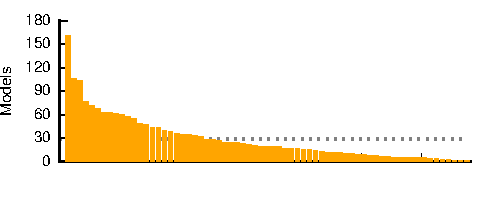
\includegraphics[width=\columnwidth]{figs/models-single-bar.pdf}\skipht
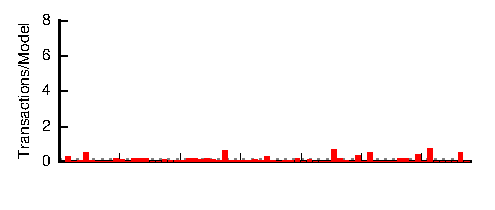
\includegraphics[width=\columnwidth]{figs/transactions-single-bar.pdf}\skipht
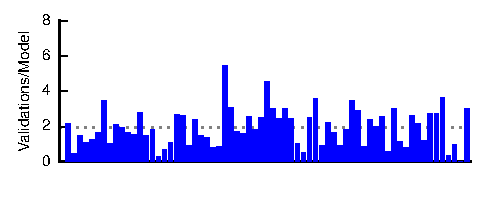
\includegraphics[width=\columnwidth]{figs/validations-single-bar.pdf}\skipht
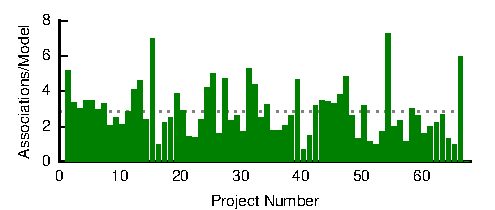
\includegraphics[width=\columnwidth]{figs/associations-single-bar.pdf}\skipht
\caption{Use of concurrency control mechanisms in Rails
  applications. Dotted line shows average for plot.}
\label{fig:usages}
\end{figure}



\minihead{Additional metrics} To better illustrate how programmers
were using each of these mechanisms, we report on two additional
analyses.

First, we analyzed the number of models, transactions, validations,
and associations over each project's lifetime. Using each
application's Git logs, we repeated the above analysis at a fixed set
of intervals through the application's history (by commits). At each
interval, we recorded the number of occurrences of each of these
constructs relative to the total number of occurences in the project
in the latest repository we examined. Figure~\ref{fig:historical}
plots the median number of occurences across all projects. Notably,
these results demonstrate that, by the time 50\% of the commits have
been entered into the repository, over 75\% of the models,
transactions, validations, and associations have been written. This
suggests that the Model layer may be less volatile than the View and
Controller components of the applications. Moreover, the initial
proportion of validations and associations is higher than the initial
proportion of transactions: the data model appears to stabilize faster
than the controller logic. It is unclear whether the bulk of
transaction usage is added in order to compensate for, say,
concurrency violations, or is instead due to growth in Controller code
and business logic.

\begin{figure}
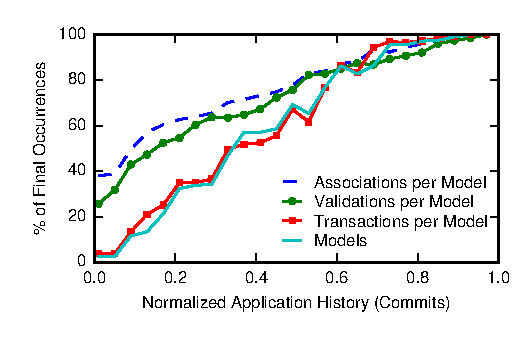
\includegraphics[width=\columnwidth]{figs/historical-median.pdf}\vspace{-2em}
\caption{Median use of Rails mechanisms over time.}
\label{fig:historical}
\end{figure}

Second, we analyze the distribution of authors to commits compared to
the distribution of authors to validations and associations
authored.\footnote{We chose to analyze commits authored rather than
  lines of code written because git tracks large-scale code
  refactoring commits as an often large set of deletions and
  insertions. Nevertheless, we observed a close correlation between
  lines of code and commits authored.} As Figure~\ref{fig:cdfs}
demonstrates, 95\% of all commits are authored by 42.4\% of
authors. However, 95\% of invariants are authored by only 20.3\% of
authors. This is reminiscent of traditional database schema
authorship, where a smaller number of authors (e.g., DBAs) modify the
schema than contribute to the actual application code.

\begin{figure}
  \newcommand{\skipht}{\\[-2em]}
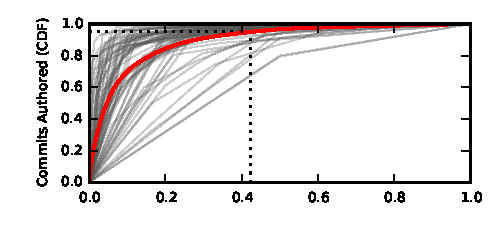
\includegraphics[width=\columnwidth]{figs/commit-authorship-cdf.pdf}\vspace{-2em}
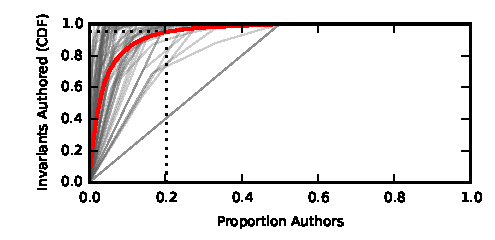
\includegraphics[width=\columnwidth]{figs/invariant-authorship-cdf.pdf}\vspace{-1em}
\caption{CDFs of authorship of invariants and commits. Bolded line
  shows the average CDF across projects, while faint lines show CDFs
  for individual projects. The dotted line shows the 95th percentile
  CDF value. }
\label{fig:cdfs}
\end{figure}

\subsection{Discussion}

Returning to the Rails design philosphy, the applications we have
encountered do indeed express their logic at the application
layer. There is little actual communication of correctness critera to
the database layer. Part of this is due to limitations within
Rails. As we have mentioned, there is no way to actually declare a
foreign key constraint in Rails without importing additional
third-party modules. Insofar as Rails is an ``opinionated'' framework
encouraging an idiomatic programming style, if our application corpus
is any indication, DHH and his co-authors advocating application-level
data management appear to have succeeded en masse.

Having observed the relative popularity of these mechanisms, we turn
our attention to the question of their correctness. Specifically, do
these application-level criteria actually enforce the constraints that
they claim to enforce? We restrict ourself to studying declared
validations and associations for three reasons. First, as we have
seen, these constructs are more widely used in the codebases we have
studied. Second, these constructs represent a deviation from standard
concurrency control techniques and are therefore perhaps more likely
to contain errors. Third, while analyzing latent constraints (i.e.,
those that might be determined via more sophisticated techniques such
as pre- and post-condition invariant
mining~\cite{writes-forest,redblue-new} and/or by interviewing each
developer on each project) would be instructive, this is difficult to
scale. We view these forms of analysis as worthwhile avenues for
future research.



\section{Isolation and Integrity}
\label{sec:apps}

We now turn our attention to understanding which of Rails' feral
validations and associations are actually correct under concurrent
execution as described in Section~\ref{sec:deployment}.

\section{Understanding Validation Behavior}

Recall that each of a model's declared validations is run before a
model instance is saved to the database. Correctly enforcing
validations requires either that \textit{i.)} validations are isolated
from one another or that \textit{ii.)} validations are somehow
``safe'' to run concurrently.

Consider the first possibility: are validations isolated? Given that
each sequence of validations (and, if validations pass, save) is
wrapped within a database-backed transaction, under serializable
isolation, validations would appear to execute correctly. However, as
is common in relational database engines~\cite{hat-vldb}, neither
PostgreSQL nor MySQL actually default to serializable isolation, and
instead provide, respectively, the weaker Read Committed and
Repeatable Read isolation levels. Under this isolation level, as we
will see shortly, many validations effectively run concurrently. While
Rails 4 does provide support for changing the isolation level on a
per-transaction basis, Rails does not actually change the database
isolation level for validations. Similarly, none of the application
code or configurations actually change the default isolation
level. Finally, we did not encounter any application deployment
documentation that suggested changing the isolation level. Although we
cannot prove that this is the case, this data suggests that
validations are likely running at default isolation in practice.

Given that validations are not likely to be perfectly isolated, does
this lack of serializable isolation actually affect these invariants?
Just because validations effectively run concurrently does not mean
that they are necessarily incorrect. To determine exactly which of
these invariants are correct under concurrent execution, we draw on
the recently developed theory of invariant
confluence~\cite{coord-avoid}.

\minihead{Methodology} Informally, invariant confluence provides a
necessary and sufficient condition for whether or not invariants can
be preserved under coordination-free, concurrent execution of
transactions. The condition effectively captures the property that
``the set of [invariant] valid states reachable by executing
transactions and merging their results is closed (w.r.t. validity)
under merge [of divergent states].'' In our MySQL and PostgreSQL
back-ends, ``merge'' of two concurrent Rails validation transactions
consists of either $i.)$ in the case of two concurrent inserts or
updates to model instances with different IDs, placing the two models
in the same table or, $ii.)$ in the case of two concurrent inserts or
updates to model instances with the same IDs, choosing an arbitrary
``winning'' write. That is, if operations $o_1$ and $o_2$ attempt to
concurrently create new model instances $i_1$ and $i_2$ with different
IDs, if each of $o_1$ and $o_2$'s validations pass, we will end up
with two new entries in the model table in the database. If $i_1$ and
$i_2$ have the same ID, we will end up with only one of the models in
the database. In the latter case, we end up with a Lost Update, but,
in general, we find that the invariants that are subject to violations
under update are similarly subject to anomalies under insertion.

Per~\cite{coord-avoid}, the state of the art in invariant confluence
analysis currently relies on a combination of manual proofs and simple
static analysis: given a set of invariant and operation pairs
classified as providing the invariant confluence property, we can
iterate through all operations and declarated invariants and check
whether or not they appear in the set of invariant confluent pairs. If
so, we can label the pair as invariant confluent. If not, we can
either conservatively label the pair as unsafe under concurrent
execution or prove the pair as invariant confluent or not. (To prove a
pair is invariant confluent, we must show that the set of database
states reachable by executing operations preserves the invariant under
merge, as described in the paragraph above.)

Returning to our task of classifying Rails validations and
associations as safe or not, we applied this invariant confluence analysis to the
validations in the corpus we examined. As~\cite{coord-avoid} observed,
many applications re-use a common set of invariants. We observed a
similar trend in our analysis of Rails applications. Recall that Rails
provides support for arbitrary, user-defined validation functions. In
fact, in our analysis, we found that only 60 out of 3551 validations
were expressed as user-defined functions. The remainder were drawn
from the standard set of validations supported by Rails
core.\footnote{It is unclear exactly why this is the case. It is
  possible that, because these invariants are standardized (in our
  case, in Rails, and, in~\cite{coord-avoid}, in SQL), they are more
  accessible to users. It is also possible that SQL and Rails have
  simply done a good job of codifying common patterns that programmers
  tend to use. This chicken-and-egg problem is an interesting subject
  for further methodological study.} Accordingly, we begin by
considering built-in validations, then examine each of these custom
validations.

\subsection{Built-In Validations}

Table~\ref{table:builtins} presents the eleven most common built-in
validations by usage and their occurences in our application
corpus.

The most popular, \texttt{presence} is multi-modal: its basic
behavior is to simply check for empty values in a model before
saving. However, it can also be used to enforce that the opposite end
of an association is, in fact, present in the database (i.e.,
referential integrity). The former use case is invariant confluent,
while the latter depends on whether or not the codebase uses deletions
or not. The second most popular invariant, \texttt{uniqueness} is
\textit{not} invariant confluent. That is, if two users concurrently
insert or modify records, they can introduce duplicates.

Eight of the next nine invariants are largely concerned with data
formatting. For example, \texttt{numericality} ensures that the field
contains a number rather than an alphanumeric string. These invariants
are indeed invariant confluent under concurrent update. Finally,
\texttt{associated} depends on whether or not the current updates are
both insertions (safe) or mixed insertions and deletions
(unsafe).

Ignoring \texttt{presence} and \texttt{associated}, we can
label 74.7\% of validation occurrences as invariant
confluent. Including these two invariants, if we mark them as not
invariant confluent (i.e., consider mixed deletions and insertions),
we have 35.2\% occurrence of invariant confluence, and, optimistically
(only considering insertions), a 87.3\% occurence of invariant
confluence invariants.

Overall, a large number of built-in validations are safe under
concurrent operation. However, associations and multi-record
uniqueness are---depending on the workload---not invariant confluent
and are therefore likely to cause problems. In the next section, we
examine these invariants in greater detail.

\begin{table}
\begin{center}
\small
\begin{tabular}{|l l l |}
\hline
Name & Occurrences & I-Confluent?\\\hline
\texttt{validates\_presence\_of} & 1764 & Depends\\
\texttt{validates\_uniqueness\_of} & 442 & No \\
\texttt{validates\_length\_of} & 302 & Yes \\
\texttt{validates\_inclusion\_of} & 167 & Yes\\
\texttt{validates\_length} & 138 & Yes \\
\texttt{validates\_format\_of} & 118 & Yes\\
\texttt{validates\_numericality\_of} & 137 & Yes \\
\texttt{validates\_format} & 69 & Yes \\
\texttt{validates\_associated} & 41 & Depends\\
\texttt{validates\_inclusion} & 36 & Yes \\
\texttt{validates\_email} & 34 & Yes \\
Other & 303 & \\\hline
\end{tabular}
\end{center}\vspace{-1em}
\caption{Use of and invariant confluence of built-in validations.}
\label{table:builtins}
\end{table}

\subsection{Custom Invariants}

We also manually inspected the coordination requirements of the 60
(1.71\%) invariants (from 17 projects) that were declared as UDFs. 52
of these were declared inline via Rails's \texttt{validates\_each}
syntax, while 8 were custom validator classes that implemented Rails's
validator interface. 42 of 60 validations were invariant confluent,
while the remaining 18 were not. For brevity, we omit a discussion of
each validator (following double-blind review, we plan to open-source
all analysis; for the time being, it \textit{is} possible to view
these validators in the wild using the open source projects and hashes
from Table~\ref{table:app-summary}) but discuss several trends and
notable examples below.

Among the custom validations that were invariant confluent, many consisted of
simple format checks or other domain-specific validation, including
credit card formatting and static username blacklisting.

The validations that were not invariant confluent took on a range of
forms. Three validations performed the equivalent of foreign key
checking, which, as we have discussed, is unsafe under deletion. Three
validations checked database-backed configuration options including
the maximum allowed file upload size and default tax rate; while
configuration updates are ostensibly rare, the outcome of each
validation could be affected under a configuration change. Two
validations were especially interesting. Spree's
\texttt{AvailabilityValidator} checks whether an eCommerce inventory
has sufficient stock available to fulfill an order; concurrent order
placement might result in negative stock. Discourse's
\texttt{PostValidator} checks whether a user has been spamming the
forum; while not necessarily critical, a spammer could technically
foil this validation by attempting to simultaneously author many posts.

In summary, again, a large class of validations appear safe. Nevertheless,
these few examples highlight the importance of protecting against
these anomalies. 





\section{Quantifying Feral Anomalies}
\label{sec:evaluation}

While many of the validations we encountered were I-confluent,
not all were. In this section, we specifically investigate the effect
of concurrent execution on two of the most popular non-I-confluent
validations: uniqueness and foreign key validations.

\subsection{Uniqueness Constraints and Isolation}

To begin, we consider Rails's uniqueness validations: 12.7\% of the
built-in validation uses we encountered. In this section, we discuss
how Rails implements uniqueness and show that this is---at least
theoretically---unsafe.

When a model field is declared with a \texttt{:validates\_uniqueness}
annotation, any instance of that model is compared against all other
corresponding records in the database to ensure that the field is
indeed unique. ActiveRecord accomplishes this by issuing a
``\texttt{SELECT}'' query in SQL and, if no such record is found,
Rails updates the instance state in the database
(Appendix~\ref{sec:appendix-uniqueness-behavior}).

While this user-level uniqueness validation runs within a transaction,
the isolation level of the transaction affects its
correctness. For correct execution, the \texttt{SELECT} query must
effectively attain a predicate lock on the validated column for the
duration of the transaction. This behavior \textit{is} supported under
serializable isolation. However, under Read Committed or Repeatable
Read isolation, no such mutual exclusion will be performed, leading to
potential inconsistency.\footnote{Using \texttt{SELECT FOR UPDATE}
  under these weaker models would be safe, but Rails does not
  implement its predicate-based lookups as such (i.e., it instead opts
  for a simple \texttt{SELECT} statement).}  Moreover, under Snapshot Isolation,
may similarly result in
inconsistency.\footnote{The first reference to the potential integrity
  violations resulting from this implementation in the Rails code that
  we are aware of dates to December 2007, in Rails
  v.2.0.0~\cite{code-unique-race-one}.  In September 2008, another
  user added additional discussion within the code comments, noting
  that ``this could even happen if you use transactions with the
  'serializable' isolation
  level''~\cite{code-unique-race-two}. Without reading too closely,
  the use of ``'serializable''' possibly suggests familiarity with the
  common, erroneous labeling of Snapshot Isolation as ``serializable''
  (as in Oracle 12c documentation and PostgreSQL documentation prior
  to the introduction of SSI in version 9.1.1 in September
  2011)\label{fn:si-rails}. } Thus, unless the database is configured
for serializable isolation, integrity violations may result.

As we have discussed, MySQL and PostgreSQL each support serializable
isolation but default to weaker isolation. Moreover, in our
investigation, we discovered a bug in PostgreSQL's implementation of
Serializable Snapshot Isolation that allowed duplicate records to be
created under serializable isolation when running a set of
transactions derived from the Rails primary key validator. We have
confirmed this anomalous behavior with the core PostgreSQL
developers\footnote{``BUG \#11732: Non-serializable outcomes under
  serializable isolation'' at
  \url{http://www.postgresql.org/message-id/20141021071458.2678.9080@wrigleys.postgresql.org}\label{fn:pg-bug}}
and, as of March 2015, the behavior persists. Thus, any discussion of
weak isolation levels aside, PostgreSQL's implementation of
serializability is non-serializable and is insufficient to provide
correct behavior for Rails' uniqueness validations. So-called
``serializable'' databases such as Oracle 12c that actually provide
Snapshot Isolation will similarly fall prey to duplicate validations.

The Rails documentation warns that uniqueness validations may fail and
admit duplicate records~\cite{rails-guide}. Yet, despite the
availability patches that remedy this behavior by the use of an
in-database constraint and/or index, Rails provides this incorrect
behavior by default. (One patch was rejected; a developer reports
``[t]he reasons for it not being incorporated...are lost in the mists
of time but I suspect it's to do with backwards compatibility, cross
database compatibility and applications varying on how they want/need
to handle these kind of errors.''~\cite{code-index-patch}).

In another bug report complaining of duplicates due to concurrent
uniqueness validation, a commenter asserts ``this is not a bug but
documented and inherent behavior of
validates\_uniqueness\_of''~\cite{code-index-error}.  A Rails
committer follows up, noting that ``the only way to handle
[uniqueness] properly is at the database layer with a unique
constraint on the column,'' and subsequently closes the issue. The
original bug reporter protests that ``the problem extends beyond
unique constraints and into validations that are unique to a Rails
application that can't [sic?!]  be enforced on the DB level''; the
Rails committer responds that ``with the possible exception of
[associations,] all of the other validations are constrained by the
attribute values currently in memory, so aren't susceptible to similar
flaws.'' This final statement is correct for many of the built-in
validations but is not correct for arbitrary user-defined
validations. We discuss the user-defined validation issue further in
Section~\ref{sec:discussion}.

\minihead{Understanding validation behavior} Given that entirely feral
mechanisms can introduce duplicates, how many duplicates can be
introduced? Once a record is written, any later validations will
observe it via \texttt{SELECT} calls. However, \textit{while} a record
is being validated, any number of concurrent validations can
unsafely proceed. In practice, the number of concurrent validations
is dependent on the Rails environment. In a Rails deployment
permitting $P$ concurrent validations (e.g., a single-threaded,
multi-process environment with $P$ processes), each value in the
domain of the model field/database column can be inserted no more than
$P$ times. Thus, validations---at least theoretically---bound the
worst-case number of duplicate records for each unique value in the
database table.

\subsection{Quantifying Uniqueness Anomalies}

Given that feral uniqueness validations are acknowledged to be unsafe
under non-serializable isolation yet are widely used, we sought to
understand exactly how often uniqueness anomalies occur in an
experimental deployment. In this section, we demonstrate that
uniqueness validations in Rails are indeed unsafe under
non-serializable isolation. While they prevent some data integrity
errors, we observe---depending on the workload---many duplicate
records.

\minihead{Experimental setup} We developed a Rails 4.1.5 application
that performed insertions to a non-indexed string column and compared
the incidence of violations both with and without a uniqueness
validator (see also
Appendix~\ref{sec:appendix-uniqueness-schema}).\footnote{In our
  experimental evaluation, we use the custom applications described
  below (and in Appendix~\ref{sec:appendix-experiments}) for two
  reasons. First, these test cases allow us to isolate ActiveRecord
  behavior to the relevant set of validations as they are deployed by
  default, independent of any specialized controller logic. Second,
  this reduces the complexity of automated testing. Many of the
  applications in our corpus indeed use the same code paths within
  ActiveRecord, but evaluating these custom applications simplifies
  programmatic triggering of validation logic.} We deployed this
application on two Amazon EC2 \texttt{m2.4xlarge} instances, offering
68.4 GB RAM, 8 CPU cores, and 1680GB local storage, running Ubuntu
14.04 LTS. On one instance, we deployed our application, using Nginx
1.6.2 as a web frontend proxied to a set of Unicorn 4.8.3 (Ruby VM
pool) workers. Nginx acts as a HTTP frontend and forwards incoming
requests to a variably sized pool of Rails VMs (managed by Unicorn, in
a multi-process, single-threaded server) that \texttt{epoll} on a
shared Linux file descriptor. On the other EC2 instance, we deployed
PostgreSQL 9.3.5 and configured it to run on the instance local
storage. We used a third EC2 instance to direct traffic to the
front-end instance and drive load. We plot the average and standard
deviation of three runs per experiment.

\minihead{Stress test} We began our study by issuing a simple stress
test that executed a number of concurrent insertion requests against a
variable number of Unicorn workers. We repeatedly issued a set of 64
concurrent model creation (SQL insertion) requests, each with the same
validated key (e.g., all with field \texttt{key} set to value 1)
against the Rails application. Across an increasing number of Unicorn
workers, we repeated this set of requests 100 times (blocking
in-between rounds to ensure that each round is, in fact, a concurrent
set of requests), changing the validated key each round
(Appendix~\ref{sec:appendix-uniqueness-stress}).

Figure~\ref{fig:pk-stress} shows the results. With no validation, all
concurrent requests succeed, resulting in 6300 duplicate records (100
rounds of 64-1 duplicate keys). With validations enabled, the number
of violations depends on the degree of concurrency allowed by
Unicorn. With only one process, Unicorn performs the validations
serially, creating no duplicates. However, with two processes, Unicorn
processes race, resulting in 70 duplicate records spread across 70
keys. With three processes, Unicorn produces 249 duplicate records
across all 100 keys. The number of duplicates increases with the
number of processes, peaking at 16 workers. With additional workers,
duplicate counts decrease slightly, which we attribute to thrashing
between workers and within PostgreSQL (recall that each instance has
only 8 cores). Nevertheless, using validations, the microbenchmark
duplicate count remains below 700---nearly an order-of-magnitude fewer
duplicates than without using validations. Therefore, even though
these validations are incorrectly implemented, they still
result in fewer anomalies. However, when we added in in-database
unique index on the \texttt{key} column\footnote{In this case, we
  added a unique index to the model using Active Record's
  \textit{database migration}, or manual schema change
  functionality. Migrations are written separately from the Active
  Record model declarations. Adding the index was not difficult, but,
  nevertheless, the index addition logic is separate from the domain
  model. Without using third-party models, we are unaware of a way to
  enforce uniqueness within Rails without first declaring an index
  that is \textit{also} annotated with a special \texttt{unique: true}
  attribute.} and repeated the experiment, we observed no duplicates,
as expected.

\begin{figure}\vspace{-1em}
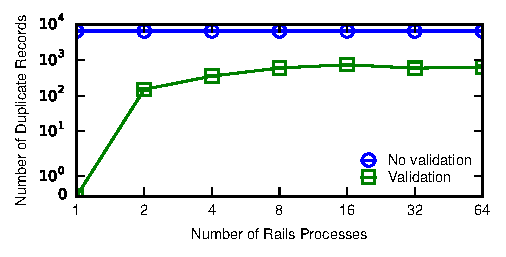
\includegraphics[width=\columnwidth]{figs/pk_stress_violations.pdf}\vspace{-1.5em}
\caption{Uniqueness stress test integrity violations.}\vspace{-.5em}
\label{fig:pk-stress}
\end{figure} 

\minihead{Actual workloads} The preceding experiment stressed a
particularly high-contention workload---in effect, a worst case
workload for uniqueness validations. In practice, such a workload is
likely rare.\footnote{In fact, it was in the above workload that we
  encountered the non-serializable PostgreSQL behavior under
  serializable isolation. Under serializable isolation, the number of
  anomalies is reduced compared to the number under Read Committed
  isolation (as we report here), but we still detected duplicate
  records.} Accordingly, we set up another workload meant to capture a
less pathological access pattern. We ran another insert-only workload,
with key choice distributed among a fixed set of keys. By varying the
distribution and number of keys, we were able to both capture more
realistic workloads and also control the amount of contention in the
workload. As a basis for comparison, we ran four different
distributions. First, we considered uniform key access. Second, we
used YCSB's Zipfian-distributed accesses from
\texttt{workloada}~\cite{ycsb}. Third and fourth, we used the item
distribution access from Facebook's LinkBench workload, which captures
MySQL record access when serving Facebook's social
graph~\cite{linkbench}. Specifically, we used---separately---the
insert and update traffic from this benchmark.

For each trial in this workload, we used 64 concurrent clients
independently issuing a set of 100 requests each, with a fixed number
of 64 Unicorn workers per process (Appendix~\ref{sec:appendix-uniqueness-workload}). 

Figure~\ref{fig:pk-workload} illustrates the number of duplicate
records observed under each of these workloads. As we increase the
number of possible keys, there are two opposing effects. With more
keys, the probability of any two operations colliding
decreases. However, recall that, once a key is written, all subsequent
validators can read it. While
the uniform workload observes an average of 2.33 duplicate records
with only one possible key, it observes an average of 26 duplicate
keys with 1000 possible keys. Nevertheless, with 1 million possible
keys, we do not observe any duplicate records.

The actual ``production'' workloads exhibit different trends. In
general, YCSB is an extremely high contention workload, with a Zipfian
constant of 0.99, resulting in one very hot key. This decreases the
beneficial effect of increasing the number of keys in the
database. However, LinkBench has less contention and anomalies decrease more
rapidly with increased numbers of keys.

\begin{figure}

\begin{minipage}[l]{0cm}

\includegraphics[angle=90, width=.185in]{figs/pk-workload-ylabel.pdf}
\end{minipage}
\begin{minipage}{\columnwidth}
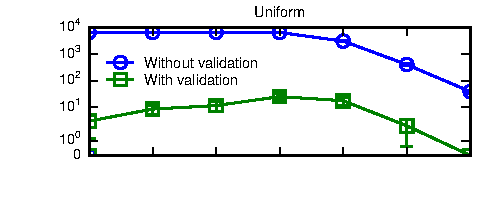
\includegraphics[width=1\columnwidth]{figs/pk-workload-uniform-violations.pdf}\vspace{-2.5em}
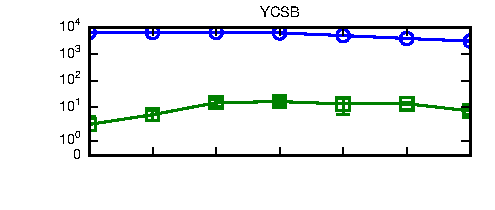
\includegraphics[width=1\columnwidth]{figs/pk-workload-ycsb-violations.pdf}\vspace{-2.5em}
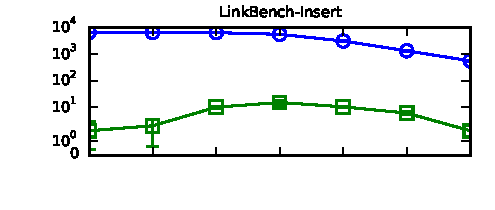
\includegraphics[width=1\columnwidth]{figs/pk-workload-linkbench-ins-violations.pdf}\vspace{-2.5em}
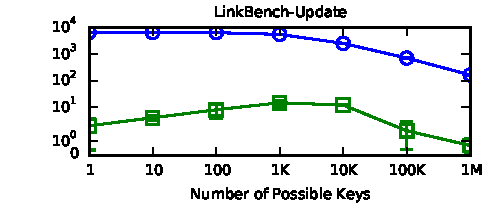
\includegraphics[width=1\columnwidth]{figs/pk-workload-linkbench-upd-violations.pdf}\vspace{-1em}
\end{minipage}
\caption{Uniqueness workload integrity violations.}\vspace{-.5em}
\label{fig:pk-workload}
\end{figure}

\subsection{Association Validations and Isolation}

Having investigated uniqueness constraints, we turn our attention to
association validations. We first, again, discuss how Rails enforces
these validations and describe how---at least
theoretically---validations might result in integrity errors.

When a model field is declared with an association (e.g., it
\texttt{:belongs\_to} another model) \textit{and} a
\texttt{:validates\_presence} validation, Rails will attempt to ensure
that the declared validation is valid before saving the model. Rails
accomplishes this by issuing a ``\texttt{SELECT WHERE}'' query in SQL
to find an associated record (e.g., to ensure the ``one'' end of a
one-to-many relationship exists) and, if a matching association is
found, Rails updates the instance state in the database
(Appendix~\ref{sec:appendix-association-behavior}). On deletion, any
models with associations marked with \texttt{:dependent => destroy}
(or \texttt{:dependent => delete}) will have any associated models
destroyed (i.e., removed by instantiating in Rails and calling
\texttt{destroy} on the model) or deleted (i.e., removed by simply
calling the database's \texttt{DELETE} method).

This feral association validation runs within a transaction, but,
again the exact isolation level of the transaction affects its
correctness. For correct execution, the \texttt{SELECT} query must
also attain a predicate lock on the specific value of the validated
column for the duration of the transaction. Similar to the uniqueness
validator, concurrent deletions and insertions are unsafe under Read
Committed, Repeatable Read, and Snapshot Isolation. Thus, unless the
database is configured for serializable isolation, inconsistency may
result and the feral validation will fail to prevent data corruption.

Unlike uniqueness validations, there is no discussion of associations
and concurrency anomalies in the Rails documentation. Moreover, in
Rails 4.1, there is no way to natively declare a foreign key
constraint;\footnote{Rails 4.2 added support for foreign keys via
  migration annotation (separate from models; similarly to adding a
  unique index) in December 2014.} it must be done via a third-party
library such as \texttt{foreigner}~\cite{foreigner} or
\texttt{schema\_plus}~\cite{schemaplus}. Only two applications
(\texttt{canvaslms} and \texttt{diaspora}) used \texttt{foreigner},
and only one application (\texttt{juvia}) used
\texttt{schema\_plus}. One application (\texttt{jobsworth}) used a
custom schema annotation and constraint generator.

\minihead{Understanding association behavior} Given that entirely
feral mechanisms can introduce broken associations, how many dangling
records can be introduced? Once a record is deleted, any later
validations will observe it via \texttt{SELECT} calls. However, in the
worst case, the feral cascading deletion on the one side of a
one-to-many relation can stall indefinitely, allowing an unlimited
number of concurrent insertions to the many side of the
relation. Thus, validations---at least theoretically---only reduce the
worst-case number of dangling records that were inserted prior to
deletion; any number of concurrent insertions may occur during
validation, leading to unbounded numbers of dangling records.

\subsection{Quantifying Association Anomalies}

Given this potential for errors, we again set out to quantify
integrity errors. We demonstrate that weak isolation can indeed lead
to data integrity errors in Rails' implementation of associations.

We performed another set of experiments to test association validation
behavior under concurrent insertions and deletions. Using the same
Unicorn and PostgreSQL deployment as above, we configured another
application to test whether or not Rails validations would correctly
enforce association-based integrity constraints. We consider an
application with two models: Users and Departments. We configure a
one-to-many relationship: each user \texttt{belongs\_to} a department,
and each department \texttt{has\_many} user
(Appendix~\ref{sec:appendix-association-schema}).

As a basic stress test, we initialize the database by creating 100
departments with no users. Subsequently, for each department in the
database, we issue a single request to delete the department along
with 64 concurrent requests to insert users in that department. To
correctly preserve the one-to-many relationship, the database should
either reject the deletion operation or perform a cascading deletion
of the department and any users (while rejecting any future user
creation requests for that department). We can quantify the degree of
inconsistency by counting the number of users left in the database who
have no corresponding department (Appendix~\ref{sec:appendix-association-stress}).

With associations declared in Rails, the Rails process performing the
deletion will attempt a cascading delete of users upon department
deletion. However, this cascade is performed, again, ferally---at the
application level. Thus, under non-serializable isolation, any user creation
events that are processed while the search for Users to delete is
underway will result in Users without departments.

Figure~\ref{fig:fk-stress} shows the number of ``orphaned'' Users
(i.e., Users without a matching Department) as a function of Rails
worker processes. With no constraints declared to Rails or to the
database, all User creations succeed, resulting in 6400 dangling
Users. With constraints declared in Rails (via a mix of validation and
association), the degree of inconsistency depends on the degree of
parallelism. Under the worst case, with 64 concurrent processes, the
validations are almost worthless in preventing integrity errors. In
contrast, when we declare a foreign key constraint within the
database\footnote{In this case, we introduced the constraint via SQL
  using a direct connection to the database. This change was
  straightforward but---like the unique index addition---was not
  reflected in the base Active Record models.}  and run the workload
again, we observe no inconsistency.

\begin{figure}
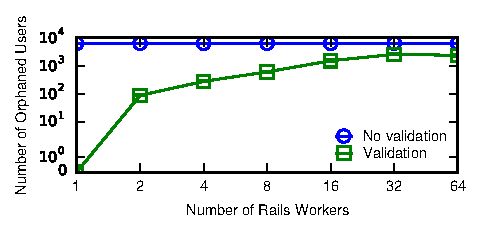
\includegraphics[width=\columnwidth]{figs/fk-stress-violations.pdf}\vspace{-1.5em}
\caption{Foreign key stress association anomalies.}\vspace{-.5em}
\label{fig:fk-stress}
\end{figure}

The above stress test shows that inconsistency due to feral
concurrency control occurs only during times of contention---parallel
deletions and insertions. We subsequently varied the degree of
contention within the workload. We configured the same application and
performed a set of insertions and deletions, but spread across a
greater number of keys and at random. A set of 64 processes
concurrently each issued 100 User creation and Department deletion
requests (at a ratio of 10 to 1) to a set of randomly-selected keys
(again at a ratio of 10 Users to each Department). By varying the
number of Users and Departments, we were able to control the amount of
contention within the workload. Under this workload, inconsistency
resulted only when a Department deletion proceeded concurrently with a
User creation event and the feral cascading deletion ``missed'' the
User creation (Appendix~\ref{sec:appendix-association-workload}).

Figure~\ref{fig:fk-workload} shows the results. As the number of
Departments increases, we observe two trends. First, with only one
Department, there is again less chance of inconsistency: all
operations contend on the same data item, so the total number of
inconsistent, orphaned users is limited by the number of potentially
racing. However, as the number of Departments increases, the chance of
concurrent deletions and insertions drops.

\begin{figure}
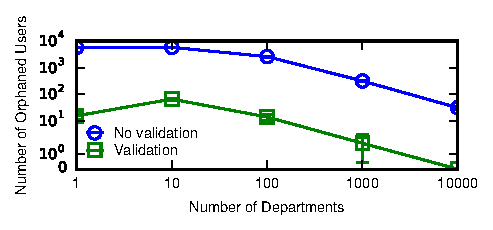
\includegraphics[width=\columnwidth]{figs/fk-workload-violations.pdf}\vspace{-1.5em}
\caption{Foreign key workload association anomalies.}\vspace{-.5em}
\label{fig:fk-workload}
\end{figure}

\subsection{Takeaways and Discussion}

The preceding experiments demonstrate that, indeed, Active Record is
unsafe as deployed by default. Validations are susceptible to data
corruption due to sensitivity to weak isolation anomalies.

This raises the question: why declare validations at all? As we
observe, validations protect against \textit{some} data
corruption. First, they correctly guard against
non-concurrency-related anomalies such as data entry or input
errors. For example, if a user attempts to reserve a username that was
previously chosen, a validation would succeed. The failures we observe
here are solely due to concurrent execution. Without concurrent
execution, validations are correct. Second, validations \textit{do}
reduce the incidence of inconsistency. Empirically, even under
worst-case workloads, these validations result in order-of-magnitude
reductions in inconsistency. Under less pathological workloads, they
may eliminate it. It is possible that, in fact, the
degree of concurrency and data contention within Rails-backed
applications simply does not lead to these concurrency races---that,
in some sense, validations are ``good enough'' for many applications.

Nevertheless, in both cases, Rails's feral mechanisms are a poor
substitute for their respective database counterparts---at least in
terms of integrity. We re-examine the Rails community's reluctance to
embrace these mechanisms in Section~\ref{sec:discussion}.




\section{Other Frameworks}
\label{sec:other-orms}

While our focus in this paper is on Rails, we briefly investigated
support for uniqueness, foreign key, and custom validations in several
other frameworks. We find widespread support for these constructs in
addition to varying degrees of susceptibility to integrity errors.

\newcommand{\orm}[1]{{\vspace{.45em}\noindent\textit{#1}}}

\orm{Java Persistence API} (JPA; version EE 7)~\cite{code-jpa} is a
standard Java Object persistence interface and supports both
uniqueness and primary key constraints in the database via specialized
object annotations. Thus, when JPA is used to create a table, it will
use the database to enforce these constraints. In 2009, JPA introduced
support for UDF validations via a JavaBean
interface~\cite{code-bean-validation}. Interestingly, both the
original (and current) Bean validation specifications specifically
address the use of uniqueness validations in their notes:
\begin{quote}
``Question: should we add @Unique that would map to @Column(unique=true)?
@Unique cannot be tested at the Java level reliably but could generate
a database unique constraint generation. @Unique is not part
of the [Bean Validation] spec today.''~\cite{jsr-bean}
\end{quote}
An author of a portion of the code specification notes separately:
\begin{quote}
  ``The reason @Unique is not part of the built-in constraints is the
  fact that accessing the [database] during a valiation [sic] is
  opening yourself up for potenital [sic] phantom reads. Think twice
  before you go for [an application-level] approach.''~\cite{unique-bean}
\end{quote}
%http://download.oracle.com/otn-pub/jcp/persistence-2.0-fr-eval-oth-JSpec/persistence-2_0-final-spec.pdf?AuthParam=1414639627_4654729130380ec6809634192c3faacb
By default, JPA Validations are run upon model save and run in a
transaction at the default isolation level, and therefore, as the
developers above hint, are susceptible to the same kinds of integrity
violations we study here.

\orm{Hibernate} (version 4.3.7)~\cite{code-hibernate}, a Java ORM
based on JPA, does \textit{not} automatically enforce declared foreign
key relationships: if a foreign key constraint is declared; a
corresponding column is added, but that column is \textit{not} backed by a
database foreign key. Instead, for both uniqueness and foreign key
constraints, Hibernate relies on JPA schema annotations for
correctness. Therefore, without appropriate schema annotations,
Hibernate's basic associations may contain dangling references. Hibernate also has an extensive user-level validation
framework implementing on the JPA Validation Bean
specification~\cite{code-hibernate-validator} and is sensitive to weak
isolation anomalies, similar to Rails validations.

\orm{CakePHP} (version 2.5.5)~\cite{code-cakephp}, a PHP-based web
framework, supports uniqueness, foreign key, and UDF
validations. CakePHP does \textit{not} back any of its validation
checking with a database transaction and relies on the user to
correctly specify any corresponding foreign keys or uniqueness
constraints within the database the schema. Thus, while users can
declare each of these validations, there is no guarantee that they are
actually enforced by the database. Thus, unless users are careful to
specify constraints in both their schema and in their validations,
validations may lead to integrity violations.

\orm{Laravel} (version 4.2)~\cite{code-laravel}, another PHP-based web
framework, supports the same set of functionality as CakePHP. Laravel
supports uniqueness, foreign key, and UDF validations in the
application, but any database-backed constraints must be specified
manually in the schema. Per one set of community documentation~\cite{laravel-book}, ``database-level
validations can efficiently handle some things (such as uniqueness of
a column in heavily-used tables) that can be difficult to implement
otherwise'' but ``[t]esting and maintenance is more difficult...[and]
your validations would be database- and schema-specific, which makes
migrations or switching to another database backend more difficult in
the future.'' In contrast, model-level validations are ``the
recommended way to ensure that only valid data is saved into your
database. They are database agnostic, cannot be bypassed by end users,
and are convenient to test and maintain.'' There
is no mention of concurrency in this current treatment, despite the
glaring potential for integrity errors.

\orm{Django} (version 1.7)~\cite{code-django}, a popular Python-based
framework, backs declared uniqueness and foreign key constraints with
database-level constraints. It also supports custom validations, but
these validations are not wrapped in a
transaction~\cite{code-django-constraints}. Thus, Django also appears
problematic, but only for custom validations.

\orm{Waterline} (version 0.10), a persistence layer for
node.js~\cite{code-waterline} (backing Sails.js, a popular MVC
framework written in Node.js~\cite{code-sails}), provides support for
in-DB foreign key and uniqueness constraints (when supported by the
database) as well as custom validations (that are \textit{not}
supported via transactions; e.g., ``TO-DO: This should all be wrapped
in a transaction. That's coming next but for the meantime just hope we
don't get in a nasty state where the operation
fails!''~\cite{code-waterline-txn}).

% Implementing and using unique indexes~\cite{waterline-unique-one,waterline-unique-two}.

\begin{comment}

Name & PK & FK & UDF Validations
DJANGO & Automatic & Automatic & Yes
JPA & Yes, annotation & Yes, annotation & Yes, via Beans
CakePHP & 

% Django

Supports validations
https://docs.djangoproject.com/en/dev/ref/validators/

Broken online: http://stackoverflow.com/a/5690705


1.9 (not yet released) deprecating in favor of checks
https://docs.djangoproject.com/en/1.7/internals/deprecation/

checks:
https://docs.djangoproject.com/en/1.7/topics/checks/



%FK 

does it right
https://docs.djangoproject.com/en/1.7/ref/models/fields/#django.db.models.ForeignKey

%PK

does it right, by default declares an index
https://docs.djangoproject.com/en/1.7/_modules/django/db/backends/schema/


'''
If True, this field must be unique throughout the table.

This is enforced at the database level and by model validation. If you try to save a model with a duplicate value in a unique field, a django.db.IntegrityError will be raised by the model’s save() method.

This option is valid on all field types except ManyToManyField, OneToOneField, and FileField.

Note that when unique is True, you don’t need to specify db_index, because unique implies the creation of an index.
'''
a

% Hibernate/JPA


%FK 

no FK by default, relies on JPA
http://docs.jboss.org/hibernate/orm/4.3/manual/en-US/html/ch08.html

JoinColumn
http://docs.oracle.com/javaee/6/api/javax/persistence/OneToMany.html

%PK

``The reason @Unique is not part of the built-in constraints is the fact that accessing the Session/EntityManager during a valiation is opening yourself up for potenital phantom reads. Think twice before you go for the following approach.''
https://developer.jboss.org/wiki/AccessingtheHibernateSessionwithinaConstraintValidator?_sscc=t
http://stackoverflow.com/questions/17092601/validate-unique-username-in-spring

http://docs.oracle.com/javaee/6/api/javax/persistence/UniqueConstraint.html

BEAN supported
https://jcp.org/en/jsr/detail?id=303

%CakePHP
supports udf validations
http://book.cakephp.org/2.0/en/models/data-validation.html

basically you set up your own schema, but default validations don't
appear to be transactional

%FK 


%PK

https://github.com/cakephp/cakephp/blob/50b3893e6507979427e1aaeb435494aed1af4f52/lib/Cake/Model/Model.php#L3303


% Laravel

Manually define database schema!

%FK 
%PK

http://laravel.com/docs/4.2/validation#rule-unique
https://github.com/laravel/framework/blob/75b1dff27778354e44511556171cf6ae466c8b59/src/Illuminate/Validation/Validator.php#L940


http://laravelbook.com/laravel-input-validation/

% Node -- Sail.js
%FK 
%PK

Validations are handled by Anchor, a thin layer on top of Validator, one of the most robust validation libraries for Node.js. Sails supports most of the validations available in Validator, as well as a few extras that require database integration, like unique.

http://sailsjs.org/#/documentation/concepts/ORM/Validations.html
https://github.com/balderdashy/sails/issues/832

https://github.com/balderdashy/waterline

Broken in Mongo
https://github.com/balderdashy/sails-mongo/issues/152

Broken in dev
https://github.com/balderdashy/waterline/issues/55

Because you have migrate: safe set the indexes will not be created when you start the ORM.
https://github.com/balderdashy/waterline/issues/236

uses db foreign keys

\end{comment}

% what can we learn?
% udfs


\section{Implications for Databases}
\label{sec:discussion}

This study highlights an important trend within common ORM systems and
ORM-backed applications: the use of feral invariants. As we have seen,
as implemented in practice, these invariants are not well-supported by
today's database systems---evidence of the continued impedance
mismatch between application writers and database systems. In light of
these findings, in this section, we reflect upon this mismatch and
make make several concrete, positive proposals for the database
systems community.

\subsection{Shortcomings Today}

Core to our findings is a lack of database support for these
feral mechanisms. In effect, today's databases effectively offer two
primary options for ORM framework developers and users:

\begin{impenumerate}
\item \textbf{Use ACID transactions.} In principle, serializable
  transactions would be sufficient to correctly enforce arbitrary
  database invariants. This is core to the transaction concept:
  isolation is a means towards preserving integrity. \vspace{.5em}

  \indent In practice, for application developers, ACID is a broken
  promise. Given its performance and availability
  overheads~\cite{brewer-cap}, developers at scale have largely
  eschewed the use of serializable transactions, which are not
  required for correct enforcement of approximately 75\% of the
  invariants we encountered in the Rails corpus. More pragmatically,
  many databases offering ``ACID'' semantics do not provide
  serializability by default and often, even among industry-standard
  enterprise offerings, offer it as an option at all~\cite{hat-vldb}
  (to say nothing of implementation difficulties, as in
  Footnote~\ref{fn:pg-bug}). Instead, these developers must manually
  reason about a host of complex, often obscure, and poorly understood
  weak isolation models expressed interms of low-level read/write
  anomalies such as Write Skew and Lost
  Update~\cite{adya-isolation,consistency-borders}. We have observed
  (e.g., Footnote~\ref{fn:si-rails}) that ORM and expert application
  developers are familiar with this mislabeling. This
  misrepresentation may even play a role in the relative unpopularity
  of transactions within the web programming community.

\item\textbf{Do it yourself (ferally).} In principle, hand-rolling
  user-level concurrency control solutions on a per-framework
  or, worse, per-application basis is an expensive, error-prone, and
  difficult process that neglects decades of intellectual achievement
  in the database community.\vspace{.5em}
  
  In practice, hand-rolling user-level concurrency control solutions
  is an expensive, error-prone, and difficult process. While this
  solution is often sufficient to maintain correctness in the
  approximately 75\% I-confluent feral invariants, the remainder
  can---in modern ORM implementations---lead to data corruption on
  behalf of applications. However, and perhaps most importantly, this
  feral approach preserves a key tenet of the Rails philosophy: a
  recurring insistence on expressing domain logic in the application.
\end{impenumerate}

In summary, neither of these solutions is good. Serializability is too
expensive for some applications, is not widely supported, and is not
necessary for many application invariants. Feral concurrency control
is often less expensive and is trivially portable but is not
sufficient for many other application invariants. In neither case does
the database respect application programmer wishes for a clean,
evidently idiomatic means of expressing correctness criteria in domain
logic.

\subsection{Domesticating Feral Mechanisms}

Constructively, we believe that, to properly provide database support
and thereby ``domesticate'' these feral mechanisms, application users
and framework authors need a new interface to the database will enable
them to:
\begin{interfaceenumerate} 
\item \textit{Express correctness criteria in the language of their
    domain model with minimal friction while permitting their
    automatic enforcement.} Per Section~\ref{sec:motivation}, a core
  factor behind the success of ORMs like Rails appears to be their
  promulgation of an idiomatic programming style that ``seems right''
  for web programming. We believe any solution to domestication must
  respect these patterns and programming style, including the ability
  to specify invariants in a framework's native language. Ideally, ORM
  programmers could enforce their existing invariants (and have them
  automatically enforced) without modification. This is already
  feasible for a subset of invariants---like uniqueness and foreign
  key constraints---but not all. An ideal solution to domestication
  would provide universal support.

\item \textit{Only pay the price of coordination when necessary.} Per
  Section~\ref{sec:apps}, many invariants can be safely executed
  without coordination, while others cannot. An ideal solution to
  domestication would enable applications to avoid coordination
  whenever possible would improve performance and operation
  availability, thus bypassing a common criticism of serializable
  transactions.

\item \textit{Easily deploy to multiple database backends.}  ORM
  frameworks today are deployed across a range of database
  implementations, and, when deciding which database features to
  exercise, framework authors often choose the least common
  denominator for compatibility purposes. An ideal solution to
  domestication would preserve this compatibility.

\end{interfaceenumerate}
While fulfilling these design requirements represents a considerable
challenge, we believe the search for a solution is both worthwhile and
of imminent practical importance.

The actual vector for implementing this interface is an open question,
but the literature lends several clues. On the one hand, we do not
believe the answer lies in exposing additional read/write isolation or
consistency guarantees like Read Committed; these fail our requirement
for an abstraction operating the level of domain logic and, as we have
noted, are challenging for developers (and researchers) to reason
about. On the other hand, more recent proposals for invariant-based
concurrency control~\cite{redblue-new,coord-avoid} and a litany of
work from prior decades on rule-based~\cite{activedb-book} and,
broadly, semantics-based concurrency control~\cite{tamer-book} appear
immediately applicable and worth (re-)considering. Recent advances in
program analysis for extracting invariants~\cite{writes-forest} and
subroutines from imperative code~\cite{statusquo} may allow us to
programatically suggest new invariants, perform correspondence
checking for existing applications, and apply a range of automated
optimizations~\cite{pyxis}. Finally, clean-slate language design and
analysis obviate the need for explicit invariant declaration (thus
alleviating concerns of specification
completeness)~\cite{calm,blazes}; while adoption within the ORM
community is a challenge, we view this exploration as worthwhile.

In all, the wide gap between research and current practice is both a
pressing concern and an exciting opportunity to revisit many decades of
research on alternatives to serializability with an eye towards
current operating conditions, application demands, and programmer
practices. Our proposal here is demanding, but so are the framework
and application writers our databases serve. While the latest
incarnation of the ORM vision may have passed over database
concurrency control, the dream is not (yet) lost.



\section{Related Work}
\label{sec:relatedwork}

There is a large body of related work that we consider in
three categories: object relational mapping systems, study of weak
isolation and applications, and the quantification of isolation behavior.

\minihead{ORMs} Database systems and application programming
frameworks have a long
history~\cite{objectstore,shore,bernstein-orm}. The ``impedance
mismatch'' between object-oriented programming and the relational
model is a perennial problem in data management systems. Ruby on Rails
is no exception, and the concurrency control issues we study here are
endemic to this mismatch---namely, disuse of common concurrency
control mechanisms like database-backed constraints. Bridging this gap
remains an active area of research~\cite{db-to-model}.

The latest wave of web programming frameworks has inspired diverse
research spanning databases, verification, and security. StatusQuo
uses program analysis and synthesis to transform imperative ORM code
into SQL, leveraging the efficiency of database-backed web
applications written in the Spring framework~\cite{statusquo}. Rails
has been the subject of study in the verification of cross-site
scripting attacks~\cite{rails-xss}, errors in data
modeling of associations~\cite{rails-bounded}, and arbitrary,
user-specified (non-validation) invariants~\cite{invariant-web}.
Rails-style ORM validations have been used to improve systems security
via client-side execution~\cite{waves,caveat}. Our focus here is on
the concurrency control requirements and usages of applications
written in Rails.

\minihead{Applications and weak isolation} The issues we examine here
are fundamental to the use of weak isolation in data management
systems. Non-serializable isolation dates to the
mid-1970s~\cite{gray-isolation} and has a colorful
history~\cite{adya-isolation}; today, by volume, most data stores are
non-serializable by default~\cite{hat-vldb}. The isolation anomalies
surfaced by the stores we study here are directly responsible for
corrupting the application data we study.

However, serializable isolation is not strictly necessary for
maintaining Rails application integrity. Semantic-based concurrency
control criteria has almost as long a lineage as
serializability~\cite{eswaran-consistency,ic-survey-two} and suggests
that, with additional, non-syntactic knowledge about applications
(e.g., integrity constraints)~\cite{kung1979optimality}, correctness
is achievable without serializability. This use of invariants has
enjoyed recent popularity in work by Li et al.~\cite{redblue-new}, Roy
et al.~\cite{writes-forest}, and Bailis et al.~\cite{coord-avoid}. We
use the concept of invariant confluence from~\cite{coord-avoid} to
determine whether Rails's built-in validators and applications written
in Rails are indeed safe under any coordination-free execution. Our
methodology is closest in spirit to~\cite{coord-avoid}, but, here, we
examine real applications instead of industrial benchmarks.

\minihead{Quantifying anomalies} A range of research similarly
quantifies the effect of non-serializable isolation in a variety of
ways.

Perhaps closest to our work is a study by Fekete et al., which
quantitatively analyzed data inconsistencies arising from
non-serializable schedules~\cite{fekete-quantifying}. This study used
a hand-crafted benchmark for analysis but is nevertheless one of the only
studies of actual application inconsistencies. Here, we focus on Rails
applications.

A larger body of work examines isolation anomalies at the read-write
interface (that is, measures deviations from properties such as
serializability or linearizability but \textit{not} the end effect of
these deviations on actual application behavior). Wada et
al. evaluated the staleness of Amazon's SimpleDB using end-user
request tracing~\cite{wada-data}, while Bermbach and Tai evaluated
Amazon S3~\cite{bermbach-eventual}, each quantifying various forms of
non-serializable behavior. Golab et al. provide algorithms for
verifying the linearizability of and sequential consistency arbitrary
data stores~\cite{golab-analyzing} and Zellag and Kemme provide
algorithms for verifying their
serializability~\cite{zellag-consistent} and other cycle-based
isolation anomalies~\cite{zellag-real}. Probabilistically Bounded
Staleness provides time- and version-based staleness predictions for
eventually consistent data stores~\cite{pbs}. While the two are
related, our focus here is on anomalies as observed by application
logic rather than read-write anomalies resulting from particular
(weak) isolation guarantees.





\section{Conclusion}
\label{sec:conclusion}

In this work, we examined the use of concurrency control mechanisms in
a set of 67 open source Ruby on Rails applications and, to a less
thorough extent, concurrency control support in a range of other web
frameworks. We found that, in contrast with traditional transaction
processing, these applications overwhelmingly prefer to leverage
application-level \textit{feral} support for data integrity, typically
in the form of declarative (sometimes user-defined) validation and
association logic. Despite the popularity of these validations, we
find limited use of in-database support to correctly implement them,
leading to a range of quantifiable inconsistencies for Rails' built-in
uniqueness and association validations. While indeed many validations
are invariant confluent and therefore correct under concurrent
execution given standard RDBMS weak isolation and concurrent update
semantics, we see considerable opportunity to better support these
users and their feral validations in the future.


\subsection*{Coda: A Call for Empiricism}

This work is a first step towards better understanding how users in
the wild actually interact with the database systems that this
community builds. Given the ascendancy of open source, there is
unprecedented opportunity to empirically and quantitatively study how
our systems are and are not serving the needs of application
programmers. Lightweight program analysis has never been easier, and
the corpus of readily-accessible code---especially in an academic
context---has never been larger.

Undoubtedly, these open source applications are dwarfed by many other
commercial and enterprise-grade codebases in terms of size, quality,
and complexity. However, compared to alternatives like TPC-C, which
today is almost 23 years old and is still the preferred benchmark for
transaction processing evaluation, open source corpuses are far better
proxies for modern applications (say, written more than a year after
the creation of the World Wide Web). Recent efforts like the
OLTPBenchmark suite~\cite{oltpbench} are a promising step forwards but
are nevertheless (and necessarily) not a substitute for real
application code. The opportunity to perform both quantitative surveys
across a large set of applications as well as longitudinal studies
over the history of each application repository (and the behavior of a
given programmer over time and repositories) are particularly
compelling. While these studies are inherently imprecise (due to
limitations of the corpus), the resulting quantitative trends are
invaluable.

In summary, in this era of ``Big Data'' analytics, we see great
promise in turning these analyses inward, towards an empirical
understanding of the usage of database systems today, in service of
better problem selection and a more quantitatively informed community
dialogue.



\scriptsize
\linespread{.98}
\selectfont

\bibliography{feral-cc} \bibliographystyle{abbrv}

\linespread{1}
\normalsize
\selectfont


\appendix


\begin{table*}
\scriptsize
\begin{tabular}{{|l}*{12}{l}{l|}}\hline
Name & Description & Authors & LoC Ruby & Commits &
 M & {\scriptsize T} & \scriptsize{PL} & \scriptsize{OL} & \scriptsize{V} &
 \scriptsize{A} & \scriptsize{Stars} &  \tiny{Githash} & \tiny{Last
   commit}\\\hline

Canvas LMS & {\scriptsize{Education}} & 132 & 308,113 & 12,889 & 161 & 46 & 12 & 1 & 354 & 839 & 1,251 & {\tiny\texttt{3fb8e69}} & {\tiny{10/16/14}}\\
OpenCongress & {\scriptsize{Congress data}} & 15 & 30,040 & 1,884 & 106 & 1 & 0 & 0 & 48 & 357 & 124 & {\tiny\texttt{850b602}} & {\tiny{02/11/13}}\\
Fedena & {\scriptsize{Education management}} & 4 & 48,359 & 1,471 & 104 & 5 & 0 & 0 & 153 & 317 & 262 & {\tiny\texttt{40cafe3}} & {\tiny{01/23/13}}\\
Discourse & {\scriptsize{Community discussion}} & 440 & 71,338 & 11,502 & 77 & 41 & 0 & 0 & 83 & 268 & 12,233 & {\tiny\texttt{1cf4a0d}} & {\tiny{10/20/14}}\\
Spree & {\scriptsize{eCommerce}} & 677 & 46,976 & 14,107 & 72 & 6 & 0 & 0 & 92 & 252 & 5,582 & {\tiny\texttt{aa34b3a}} & {\tiny{10/16/14}}\\
Sharetribe & {\scriptsize{Content management}} & 35 & 30,357 & 7,140 & 68 & 0 & 0 & 0 & 112 & 202 & 127 & {\tiny\texttt{8e0d382}} & {\tiny{10/21/14}}\\
ROR Ecommerce & {\scriptsize{eCommerce}} & 19 & 16,732 & 1,604 & 63 & 2 & 3 & 0 & 219 & 207 & 857 & {\tiny\texttt{c60a675}} & {\tiny{10/09/14}}\\
Diaspora & {\scriptsize{Social network}} & 388 & 31,361 & 14,640 & 63 & 2 & 0 & 0 & 66 & 128 & 9,571 & {\tiny\texttt{1913397}} & {\tiny{10/03/14}}\\
Redmine & {\scriptsize{Project management}} & 10 & 79,483 & 11,049 & 62 & 11 & 0 & 1 & 131 & 157 & 2,264 & {\tiny\texttt{e23d4d9}} & {\tiny{10/19/14}}\\
ChiliProject & {\scriptsize{Project management}} & 53 & 64,512 & 5,532 & 61 & 7 & 0 & 1 & 118 & 130 & 623 & {\tiny\texttt{984c9ff}} & {\tiny{08/13/13}}\\
Spot.us & {\scriptsize{Community reporting}} & 46 & 92,737 & 9,280 & 58 & 0 & 0 & 0 & 96 & 165 & 343 & {\tiny\texttt{61b65b6}} & {\tiny{12/02/13}}\\
Jobsworth & {\scriptsize{Project management}} & 46 & 24,469 & 7,890 & 55 & 10 & 0 & 0 & 86 & 225 & 478 & {\tiny\texttt{3a1f8e1}} & {\tiny{09/12/14}}\\
OpenProject & {\scriptsize{Project management}} & 63 & 82,764 & 11,185 & 49 & 8 & 1 & 3 & 136 & 227 & 371 & {\tiny\texttt{c1e66af}} & {\tiny{11/21/13}}\\
Danbooru & {\scriptsize{Image board}} & 25 & 27,812 & 3,738 & 47 & 9 & 0 & 0 & 71 & 114 & 238 & {\tiny\texttt{c082ed1}} & {\tiny{10/17/14}}\\
Salor Retail & {\scriptsize{Point of Sale}} & 26 & 18,007 & 2,259 & 44 & 0 & 0 & 0 & 81 & 309 & 24 & {\tiny\texttt{00e1839}} & {\tiny{10/07/14}}\\
Zena & {\scriptsize{Content management}} & 7 & 55,694 & 2,514 & 44 & 1 & 0 & 0 & 12 & 43 & 172 & {\tiny\texttt{79576ac}} & {\tiny{08/18/14}}\\
Skyline CMS & {\scriptsize{Content management}} & 7 & 10,241 & 894 & 40 & 5 & 0 & 0 & 28 & 89 & 127 & {\tiny\texttt{64b0932}} & {\tiny{12/09/13}}\\
Opal & {\scriptsize{Project management}} & 6 & 10,643 & 474 & 38 & 3 & 0 & 0 & 42 & 96 & 45 & {\tiny\texttt{11edf34}} & {\tiny{01/09/13}}\\
OneBody & {\scriptsize{Church portal}} & 33 & 19,867 & 3,976 & 36 & 3 & 0 & 0 & 97 & 140 & 1,041 & {\tiny\texttt{2dfbd4d}} & {\tiny{10/19/14}}\\
CommunityEngine & {\scriptsize{Social networking}} & 67 & 13,796 & 1,613 & 35 & 3 & 0 & 0 & 92 & 101 & 1,073 & {\tiny\texttt{a4d3ea2}} & {\tiny{10/16/14}}\\
Publify & {\scriptsize{Blogging}} & 93 & 16,555 & 5,067 & 35 & 7 & 0 & 0 & 33 & 50 & 1,274 & {\tiny\texttt{4acf86e}} & {\tiny{10/20/14}}\\
Comas & {\scriptsize{Conference management}} & 5 & 6,893 & 435 & 33 & 6 & 0 & 0 & 80 & 45 & 21 & {\tiny\texttt{81c25a4}} & {\tiny{09/09/14}}\\
BrowserCMS & {\scriptsize{Content management}} & 56 & 21,011 & 2,503 & 32 & 4 & 0 & 0 & 47 & 77 & 1,183 & {\tiny\texttt{d654557}} & {\tiny{09/30/14}}\\
RailsCollab & {\scriptsize{Project managment}} & 25 & 8,799 & 865 & 29 & 6 & 0 & 0 & 40 & 122 & 262 & {\tiny\texttt{9f6c8c1}} & {\tiny{02/16/12}}\\
Insoshi & {\scriptsize{Social network}} & 16 & 118,619 & 1,321 & 28 & 2 & 0 & 0 & 63 & 164 & 1,583 & {\tiny\texttt{9976cfe}} & {\tiny{02/24/10}}\\
OpenGovernment & {\scriptsize{Government data}} & 15 & 8,906 & 2,231 & 28 & 4 & 0 & 0 & 22 & 141 & 160 & {\tiny\texttt{fa80204}} & {\tiny{11/21/13}}\\
Tracks & {\scriptsize{Personal productivity}} & 89 & 17,312 & 3,121 & 27 & 2 & 0 & 0 & 24 & 43 & 639 & {\tiny\texttt{eb2650c}} & {\tiny{10/02/14}}\\
GitLab & {\scriptsize{Code management}} & 672 & 37,671 & 12,319 & 24 & 15 & 0 & 0 & 131 & 114 & 14,129 & {\tiny\texttt{72abe9f}} & {\tiny{10/20/14}}\\
Brevidy & {\scriptsize{Video sharing}} & 2 & 7,118 & 6 & 24 & 1 & 0 & 0 & 74 & 56 & 167 & {\tiny\texttt{d0ddb1a}} & {\tiny{01/18/14}}\\
Alchemy & {\scriptsize{Content management}} & 34 & 19,097 & 4,222 & 23 & 2 & 0 & 0 & 37 & 40 & 240 & {\tiny\texttt{91d9d08}} & {\tiny{10/20/14}}\\
Teambox & {\scriptsize{Project management}} & 48 & 32,252 & 3,155 & 22 & 2 & 0 & 0 & 56 & 116 & 1,864 & {\tiny\texttt{62a8b02}} & {\tiny{09/20/11}}\\
Fat Free CRM & {\scriptsize{Customer relationship}} & 99 & 20,754 & 4,144 & 21 & 3 & 0 & 0 & 39 & 92 & 2,384 & {\tiny\texttt{3dd2c62}} & {\tiny{10/17/14}}\\
linuxfr.org & {\scriptsize{FLOSS community}} & 29 & 8,060 & 2,271 & 20 & 1 & 0 & 0 & 50 & 50 & 86 & {\tiny\texttt{5d4d6df}} & {\tiny{10/14/14}}\\
Squash & {\scriptsize{Bug reporting}} & 28 & 15,663 & 231 & 19 & 6 & 0 & 0 & 87 & 62 & 879 & {\tiny\texttt{c217ac1}} & {\tiny{09/15/14}}\\
Shoppe & {\scriptsize{eCommerce}} & 14 & 3,115 & 349 & 19 & 1 & 0 & 0 & 58 & 34 & 208 & {\tiny\texttt{19e60c8}} & {\tiny{10/18/14}}\\
nimbleShop & {\scriptsize{eCommerce}} & 12 & 7,513 & 1,805 & 19 & 0 & 0 & 0 & 47 & 34 & 47 & {\tiny\texttt{4254806}} & {\tiny{02/18/13}}\\
Piggybak & {\scriptsize{eCommerce}} & 16 & 2,205 & 383 & 17 & 1 & 0 & 0 & 51 & 35 & 166 & {\tiny\texttt{2bed094}} & {\tiny{09/10/14}}\\
wallgig & {\scriptsize{Wallpaper sharing}} & 6 & 5,541 & 350 & 17 & 1 & 0 & 0 & 42 & 45 & 18 & {\tiny\texttt{4424d44}} & {\tiny{03/23/14}}\\
Rucksack & {\scriptsize{Collaboration}} & 7 & 5,309 & 445 & 17 & 3 & 0 & 0 & 18 & 79 & 169 & {\tiny\texttt{59703d3}} & {\tiny{10/05/13}}\\
Calagator & {\scriptsize{Online calendar}} & 48 & 8,877 & 1,766 & 16 & 0 & 0 & 0 & 8 & 11 & 196 & {\tiny\texttt{6e5df08}} & {\tiny{10/19/14}}\\
Amahi Platform & {\scriptsize{Home media sharing}} & 15 & 6,187 & 577 & 15 & 2 & 0 & 0 & 38 & 22 & 65 & {\tiny\texttt{5101c8b}} & {\tiny{08/20/14}}\\
Sprint & {\scriptsize{Project management}} & 5 & 3,053 & 71 & 14 & 0 & 0 & 0 & 50 & 45 & 247 & {\tiny\texttt{584d887}} & {\tiny{09/17/14}}\\
Citizenry & {\scriptsize{Community directory}} & 17 & 7,939 & 512 & 13 & 0 & 0 & 0 & 12 & 45 & 138 & {\tiny\texttt{e314fe4}} & {\tiny{04/01/14}}\\
Saasy & {\scriptsize{eCommerce}} & 2 & 161,092 & 21 & 12 & 5 & 0 & 0 & 41 & 117 & 520 & {\tiny\texttt{4fe610f}} & {\tiny{08/03/09}}\\
LovdByLess & {\scriptsize{Social network}} & 17 & 29,639 & 150 & 12 & 0 & 0 & 0 & 27 & 41 & 568 & {\tiny\texttt{26e79a7}} & {\tiny{10/09/09}}\\
lobste.rs & {\scriptsize{Link sharing}} & 24 & 4,927 & 624 & 12 & 8 & 0 & 0 & 20 & 40 & 646 & {\tiny\texttt{b0b9654}} & {\tiny{10/18/14}}\\
BucketWise & {\scriptsize{Personal finance}} & 10 & 4,343 & 258 & 12 & 2 & 0 & 0 & 11 & 46 & 484 & {\tiny\texttt{5c73f2b}} & {\tiny{06/10/12}}\\
Sugar & {\scriptsize{Forum}} & 13 & 7,590 & 1,316 & 11 & 1 & 0 & 0 & 20 & 53 & 89 & {\tiny\texttt{49ca79f}} & {\tiny{10/21/14}}\\
Comfy Mexican Sofa & {\scriptsize{Content management}} & 106 & 8,831 & 1,748 & 10 & 0 & 0 & 0 & 35 & 26 & 1,523 & {\tiny\texttt{fecef0c}} & {\tiny{10/09/14}}\\
Radiant & {\scriptsize{Content management}} & 100 & 15,124 & 2,385 & 9 & 3 & 0 & 1 & 26 & 12 & 1,554 & {\tiny\texttt{0c9ef9b}} & {\tiny{10/01/14}}\\
Refinery CMS & {\scriptsize{Content management}} & 438 & 10,797 & 9,112 & 9 & 0 & 0 & 0 & 16 & 8 & 2,979 & {\tiny\texttt{f4e24ef}} & {\tiny{10/20/14}}\\
Forem & {\scriptsize{Forum}} & 106 & 4,632 & 1,409 & 9 & 0 & 0 & 0 & 10 & 29 & 1,302 & {\tiny\texttt{519f2de}} & {\tiny{08/14/14}}\\
BostonRB & {\scriptsize{Ruby community}} & 40 & 2,128 & 889 & 7 & 0 & 0 & 0 & 18 & 12 & 199 & {\tiny\texttt{05fc100}} & {\tiny{10/21/14}}\\
Inkwell & {\scriptsize{Social networking}} & 6 & 6,731 & 156 & 7 & 0 & 0 & 0 & 4 & 51 & 327 & {\tiny\texttt{d1938d3}} & {\tiny{07/15/14}}\\
Boxroom & {\scriptsize{File sharing}} & 9 & 1,924 & 368 & 6 & 0 & 0 & 0 & 18 & 12 & 218 & {\tiny\texttt{1e74e06}} & {\tiny{10/18/14}}\\
Copycopter & {\scriptsize{Copy writing}} & 9 & 2,267 & 46 & 6 & 1 & 0 & 0 & 7 & 14 & 652 & {\tiny\texttt{d3607c4}} & {\tiny{06/28/12}}\\
Enki & {\scriptsize{Blogging}} & 29 & 4,584 & 562 & 6 & 1 & 0 & 0 & 5 & 7 & 835 & {\tiny\texttt{b793d48}} & {\tiny{12/01/13}}\\
Fulcrum & {\scriptsize{Project planning}} & 46 & 3,054 & 637 & 5 & 0 & 0 & 0 & 13 & 15 & 1,335 & {\tiny\texttt{8397de2}} & {\tiny{08/20/14}}\\
GitLab CI & {\scriptsize{Continuous integration}} & 80 & 3,650 & 870 & 5 & 2 & 0 & 0 & 11 & 13 & 1,188 & {\tiny\texttt{7d51134}} & {\tiny{10/17/14}}\\
Kandan & {\scriptsize{Persistent chat}} & 56 & 1,533 & 808 & 5 & 0 & 0 & 0 & 6 & 8 & 2,249 & {\tiny\texttt{15a8aab}} & {\tiny{10/06/14}}\\
Juvia & {\scriptsize{Commenting}} & 8 & 2,280 & 202 & 4 & 3 & 0 & 0 & 11 & 8 & 937 & {\tiny\texttt{43a1c48}} & {\tiny{05/09/14}}\\
Go vs Go & {\scriptsize{Go board game}} & 2 & 2,317 & 302 & 4 & 0 & 0 & 0 & 11 & 9 & 145 & {\tiny\texttt{c8d739d}} & {\tiny{02/21/13}}\\
Adopt-a-Hydrant & {\scriptsize{Civics}} & 14 & 14,163 & 1,242 & 3 & 0 & 0 & 0 & 11 & 8 & 182 & {\tiny\texttt{5b7ea0e}} & {\tiny{10/21/14}}\\
Selfstarter & {\scriptsize{Crowdfunding}} & 23 & 574 & 127 & 3 & 0 & 0 & 0 & 1 & 4 & 2,688 & {\tiny\texttt{740075f}} & {\tiny{05/16/14}}\\
Heaven & {\scriptsize{Code deployment}} & 19 & 2,083 & 387 & 2 & 0 & 0 & 0 & 2 & 2 & 163 & {\tiny\texttt{2d4162e}} & {\tiny{10/21/14}}\\
Carter & {\scriptsize{eCommerce}} & 3 & 1,052 & 70 & 2 & 1 & 0 & 0 & 0 & 12 & 22 & {\tiny\texttt{60ad49d}} & {\tiny{07/22/14}}\\
Obtvse & {\scriptsize{Blogging}} & 27 & 427 & 393 & 1 & 0 & 0 & 0 & 3 & 0 & 1,516 & {\tiny\texttt{1542856}} & {\tiny{03/21/13}}\\\hline
\textbf{Average:} &  & \textbf{69.21} & \textbf{26,380.48} & \textbf{2,953.31} & \textbf{29.21} & \textbf{3.87} & \textbf{0.24} & \textbf{0.10} & \textbf{53.00} & \textbf{96.04} & \textbf{1,272.42} &  & {\tiny\textbf{02/06/14}}\\

\hline
\end{tabular}
\caption{Corpus of applications used in analysis (M: Models, T:
  Transactions, PL: Pessimistic Locking, OL: Optimistic Locking, V:
  Validations, A: Associations). Stars record number of GitHub Stars
  as of October 2014.}
\label{table:app-summary}
\end{table*}

\section{Analysis Methodology}
\subsection{Mechanism Analysis}
\label{sec:appendix-methodology}

To determine the occurrences and number of models, transactions, locks, validations, and associations in Rails, we used a very simple set of custom code analysis scripts. We do not consider the analysis techniques here a contribution; rather, our interest is in the output of the analysis.  (Though we hesitate to term this process ``program analysis,'' the scripts embody a very simple syntactic static analysis.) The syntactic approach proved portable between the many versions of Rails against which each application is linked; otherwise, porting between non-backwards-compatible Rails versions was difficult and, in fact, unsupported by several of the Rails code analysis tools we considered using as alternatives. The choice to use syntax as a means of distinguishing code constructs led to some ambiguity. To compensate, we introduced custom logic to handle esoteric syntaxes that arose in particular projects (e.g., some projects extend \texttt{ActiveRecord::Base} with a separate, project-specific base class, while some validation usages vary between constructs like \texttt{:validates\_presence} and \texttt{:validates\_presence\_of}).

To determine code authorship, we used the output of git \texttt{log} and \texttt{blame} and did not attempt any sophisticated entity resolution.


\subsection{Invariant Confluence}
\label{sec:appendix-ic}

Overall, our I-confluence analysis was relatively straightforward, and is similar to that of~\cite{coord-avoid} (in fact, many of the results from prior work, such as uniqueness constraints and foreign key constraints have already been classified). The primary incidence of non-pre-classified invariant-operation pairs came from data formatting constraints, but these closely resemble the ``Attribute Equality'' constraints considered in~\cite[Proof 1]{coord-avoid}. ActiveRecord is actually fairly easy to analyze in this manner as the entire write set is simply the model instance to be saved.

\section{Detailed Validation Behavior}

\subsection{Uniqueness Validation}
\label{sec:appendix-uniqueness-behavior}

When a controller attempts to \texttt{save} an ActiveRecord model instance $i$ of type $M$, if $M$ has a declared \texttt{:validates\_uniqueness} annotation on attribute $a$, the following steps will be performed during validation:

\begin{enumerate} 
\small

\item Assuming that instances of $M$ are stored in database table $T_M$ (with attribute $a$ stored in column $C_a$), Active Record will perform the equivalent of $$\texttt{SELECT 1 FROM $T_M$ where $C_a$ = $i.a$ LIMIT ONE;}$$ (\texttt{SELECT COUNT(*)} would be sufficient here as well, but this is not how the query is actually implemented).

\item If this result set is empty, the validation succeeds.

\item If this result set is not empty, the validation fails. If the validation was called during \texttt{save}, it returns \texttt{false}. If the validation was called during \texttt{save!}, it raises an \texttt{ActiveRecord::RecordInvalid} exception.

\end{enumerate}

This is a classic example of the phantom problem. As we mention in Section~\ref{sec:evaluation}, changing this \texttt{SELECT} call to \texttt{SELECT FOR UPDATE} would be sufficient (given an appropriate implementation of next-key locking). However, Rails is not implemented as such.

\subsection{Association Validation}
\label{sec:appendix-association-behavior}

 When a controller attempts to \texttt{save} an ActiveRecord model instance $i$ of type $M$, if $M$ has a declared \texttt{:belongs\_to} annotation on attribute $a$ pointing to attribute $b$ of model $N$ \textit{and} $M$ has a declared \texttt{:validates\_presence} annotation on attribute $a$, the following steps will be performed during validation:

\begin{enumerate} 
\small
\item Assuming that instances of $N$ are stored in database table $T_N$ (with attribute $b$ stored in column $C_b$), Active Record will perform the equivalent of $$\texttt{SELECT 1 FROM $T_N$ where $C_b$ = $i.a$ LIMIT ONE;}$$

\item If this result set is not empty, the validation succeeds.

\item If this result set is empty, the validation fails. If the validation was called during \texttt{save}, it returns \texttt{false}. If the validation was called during \texttt{save!}, it raises an \texttt{ActiveRecord::RecordInvalid} exception.

\end{enumerate}

\section{Experimental Description}
\label{sec:appendix-experiments}

\lstset{language=Ruby,basicstyle=\ttfamily\small,columns=fullflexible,frame=single}

We describe our applications from Section~\ref{sec:evaluation} in greater detail.

\subsection{Uniqueness Validation Schema}
\label{sec:appendix-uniqueness-schema}

We declare two models, each containing two attributes: \texttt{key}, a string, and \texttt{value}, also a string. The generated schema for each of the models, which we call \texttt{SimpleKeyValue} and \texttt{ValidatedKeyValue}, is the same. The schema for \texttt{SimpleKeyValue} is as follows:

\begin{lstlisting}
  create_table "validated_key_values", force: true do |t|
    t.string   "key"
    t.string   "value"
    t.datetime "created_at"
    t.datetime "updated_at"
  end
\end{lstlisting}

For the non-uniqueness-validated model, we simply require that the \texttt{key} and \texttt{value} fields are not null:

\begin{lstlisting}
class SimpleKeyValue < ActiveRecord::Base
  validates :key, presence: true
  validates :value, presence: true
end
\end{lstlisting}

For \texttt{ValidatedKeyValue}, we add a \texttt{uniqueness} constraint to the \texttt{key} field.

\begin{lstlisting}
class ValidatedKeyValue < ActiveRecord::Base
  validates :key, presence: true, uniqueness: true
  validates :value, presence: true
end
\end{lstlisting}

The remainder of the application consists of a simple View and Controller logic to allow us to \texttt{POST}, \texttt{GET}, and \texttt{DELETE} each kind of model instance programatically via HTTP.


\subsection{Uniqueness Stress Test}
\label{sec:appendix-uniqueness-stress}

For the uniqueness stress test (Figure~\ref{fig:pk-stress}), we repeatedly attempt to create duplicate records. We issue a set of 64 concurrent requests to create instances with the \texttt{key} field set to an increasing sequence number ($k$, below) and repeat 100 times. At the end of the run, we count the number of duplicate records in the table:

\begin{algorithm}[H]
\begin{algorithmic}
\For{model $m \in \{\texttt{SimpleKeyValue}, \texttt{ValidatedKeyValue}\}$}
  \For{$k \gets 1$ to $100$}
    \ParFor{$1$ to $64$}
      \State via HTTP: create new $m$ with \texttt{key=$k$}
     \EndParFor
   \EndFor
   \State dups $\gets $execute(\texttt{SELECT key, COUNT(key)-1 FROM $T_M$}
   \State \hspace{6.5em}\texttt{GROUP BY key HAVING COUNT(key) > 1;})
\EndFor
\end{algorithmic}
\end{algorithm}

Under correct validation, all but one of the creation requests per key should fail.

\subsection{Uniqueness Workload Test}
\label{sec:appendix-uniqueness-workload}

For the uniqueness workload test (Figure~\ref{fig:pk-workload}), a set of 64 workers sequentially issues a set of 100 operations each. Each operation attempts to create a new model instance with the \texttt{key} field set to a random item generated according to the distributions described in Section~\ref{sec:evaluation}:

\begin{algorithm}[H]
\begin{algorithmic}
\For{model $m \in \{\texttt{SimpleKeyValue}, \texttt{ValidatedKeyValue}\}$}
  \ParFor{$1$ to $64$}
    \For{$1$ to $100$}
      \State $k \gets$ \textit{pick new key according to distribution}
      \State via HTTP: create new $m$ with \texttt{key=$k$}
     \EndFor
   \EndParFor
   \State dups $\gets $execute(\texttt{SELECT key, COUNT(key)-1 FROM $T_M$}
   \State \hspace{6.5em}\texttt{GROUP BY key HAVING COUNT(key) > 1;})
\EndFor
\end{algorithmic}
\end{algorithm}

\subsection{Association Validation Schema}
\label{sec:appendix-association-schema}

We declare two sets of models, each containing two models each: a \texttt{User} model and a \texttt{Departments} model. Each \texttt{User} has a(n implicit) \texttt{id} (as generated by Rails ActiveRecord) and an integer corresponding \texttt{department\_i}. Each \texttt{Department} has an \texttt{id}. Both models have a timestamp of the last updated and creation time, as is auto-generated by Rails. Aside from the table names, both schemas are equivalent. Below is the schema for the non-validated users and departments:
\begin{lstlisting}
create_table "simple_users", force: true do |t|
    t.integer  "simple_department_id"
    t.datetime "created_at"
    t.datetime "updated_at"
end

create_table "simple_departments", force: true do |t|
  t.datetime "created_at"
  t.datetime "updated_at"
end
\end{lstlisting}
The two pairs of models vary in their validations. One pair of models has no validations or associations:
\begin{lstlisting}
class SimpleDepartment < ActiveRecord::Base
end

class SimpleUser < ActiveRecord::Base
end
\end{lstlisting}
The other pair of models contain validations, including rules for cascading deletions (note that we only delete from Departments in our workload, below):
\begin{lstlisting}
class ValidatedDepartment < ActiveRecord::Base
  has_many :validated_users, :dependent => :destroy
end

class ValidatedUser < ActiveRecord::Base
  belongs_to :validated_department
  validates :validated_department, :presence => true
end
\end{lstlisting}
Thus, on deletion of a model of type \texttt{ValidatedDepartment}, ActiveRecord will attempt to call \texttt{destroy} on each matching \texttt{ValidatedUser}.

\subsection{Association Stress Test}
\label{sec:appendix-association-stress}

For the association stress test (Figure~\ref{fig:fk-stress}), we repeatedly attempt to create orphan users. We issue a set of 64 concurrent requests to create Users belonging to a particular department, while simultaneously deleting that department and repeat 100 times. At the end of the run, we count the number of users with a department that does not exist:

\begin{algorithm}[H]
\begin{algorithmic}
\For{model $m \in \{\texttt{Simple}, \texttt{Validated}\}$}
  \For{$i \gets 1$ to $100$}
    \State via HTTP: create $m$Department with \texttt{id=$i$}
  \EndFor
  \For{$i \gets 1$ to $100$}
    \ParFor{$w \in 1$ to $65$}
      \If {$w = 1$}
        \State via HTTP: delete $m$Department with \texttt{id=$i$}
      \Else
        \State via HTTP: create new $m$User \texttt{department\_id=$i$}
      \EndIf        
     \EndParFor
   \EndFor
   \State orphaned $\gets $execute(``\texttt{SELECT $m$\_department\_id,}
   \State \hspace{8.5em}\texttt{COUNT(*) FROM $m$\_users AS U}
   \State \hspace{8.5em}\texttt{LEFT OUTER JOIN}
   \State \hspace{8.5em}\texttt{$m$\_departments AS D}
   \State \hspace{8.5em}\texttt{ON U.$m$\_department\_id = D.id}
   \State \hspace{8.5em}\texttt{WHERE D.id IS NULL}
   \State \hspace{8.5em}\texttt{GROUP BY $m$\_department\_id}
   \State \hspace{8.5em}\texttt{HAVING COUNT(*) > 0;}'')
\EndFor
\end{algorithmic}
\end{algorithm}

\subsection{Association Workload Test}
\label{sec:appendix-association-workload}

For the association workload test (Figure~\ref{fig:fk-workload}), we begin by creating a variable number of departments (Figure~\ref{fig:fk-workload} x-axis; $D$). We next have 64 concurrent clients simultaneously attempt to create users belonging to a random department and delete random departments (in a 10:1 ratio of creations to deletions, for 100 operations each). We end by counting the number of orphaned users, as above.

\begin{algorithm}[H]
\begin{algorithmic}
\For{model $m \in \{\texttt{Simple}, \texttt{Validated}\}$}
  \For{$d \gets 1$ to $D$}
    \State via HTTP: create $m$Department with \texttt{id=$i$}
  \EndFor
  \ParFor{$w \in 1$ to $64$}
      \State $d \gets uniformRandomInt([1, D])$
      \If {$uniformRandomDouble([0, 1]) < \frac{1}{11}$}
        \State via HTTP: delete $m$Department with \texttt{id=$d$}
      \Else
        \State via HTTP: create new $m$User \texttt{department\_id=$d$}
      \EndIf        
   \EndParFor
   \State orphaned $\gets $ as above, in stress test
\EndFor
\end{algorithmic}
\end{algorithm}


\balance


\end{document}
